% ****** Start of file apssamp.tex ******
%
%   This file is part of the APS files in the REVTeX 4.2 distribution.
%   Version 4.2a of REVTeX, December 2014
%
%   Copyright (c) 2014 The American Physical Society.
%
%   See the REVTeX 4 README file for restrictions and more information.
%
% TeX'ing this file requires that you have AMS-LaTeX 2.0 installed
% as well as the rest of the prerequisites for REVTeX 4.2
%
% See the REVTeX 4 README file
% It also requires running BibTeX. The commands are as follows:
%
%  1)  latex apssamp.tex
%  2)  bibtex apssamp
%  3)  latex apssamp.tex
%  4)  latex apssamp.tex
%
\documentclass[%
 preprint, linenumbers,
%superscriptaddress,
%groupedaddress,
%unsortedaddress,
%runinaddress,
%frontmatterverbose, 
%preprint,
%preprintnumbers,
%nofootinbib,
%nobibnotes,
%bibnotes,
 amsmath,amssymb,
 aps, physrev,
%pra,
%prb,
%rmp,
%prstab,
%prstper,
%floatfix,
]{revtex4-2}

\usepackage{graphicx}% Include figure files
\usepackage{dcolumn}% Align table columns on decimal point
\usepackage{bm}% bold math
\usepackage{braket} % For \bra{}, \ket{} and \braket{}
%\usepackage{hyperref}% add hypertext capabilities
%\usepackage[mathlines]{lineno}% Enable numbering of text and display math
%\linenumbers\relax % Commence numbering lines


%\usepackage[showframe,%Uncomment any one of the following lines to test 
%%scale=0.7, marginratio={1:1, 2:3}, ignoreall,% default settings
%%text={7in,10in},centering,
%%margin=1.5in,
%%total={6.5in,8.75in}, top=1.2in, left=0.9in, includefoot,
%%height=10in,a5paper,hmargin={3cm,0.8in},
%]{geometry}
\usepackage{float}
\begin{document}

\preprint{APS/123-QED}

\title{\textbf{ Spin in Density-Functional Theory.} 
}% 


 
\author{Aury Castro}
 \email{Aury.castro@unipamplona.edu}
\affiliation{ Universidad de pamplona\\}



\begin{abstract}
 This article delves into the incorporation of spin within Density Functional Theory (DFT), emphasizing its pivotal role in understanding electronic systems. Starting with foundational concepts from nonrelativistic quantum mechanics, the discussion evolves to include the Hohenberg–Kohn theorems and their generalization for spin-dependent systems. Furthermore, the manuscript explores the Kohn–Sham formulation, contrasting spin-restricted and spin-unrestricted frameworks. Through these analyses, the study addresses critical challenges, such as spin contamination and the limitations of approximate functionals, proposing a roadmap to improve the treatment of spin in open-shell systems and magnetic materials. This work provides insights into the theoretical advancements and computational approaches necessary to tackle the complexities of spin-dependent electronic interactions.
\end{abstract}

%\keywords{Suggested keywords}%Use showkeys class option if keyword
                              %display desired
\maketitle


\section{Introduction}
Density functional theory (DFT) is one of the most widely used methods in computational chemistry and solid-state physics to describe electronic systems. However, the correct incorporation of spin, an intrinsic property of electrons, has posed fundamental theoretical and practical challenges. The quantum nature of spin directly affects electron-electron interactions and magnetic properties of systems, especially in magnetic materials and open-shell systems.

This article examines the treatment of spin in DFT from a theoretical perspective, starting with its description in non-relativistic quantum mechanics and moving towards specific developments in the contexts of the Hohenberg–Kohn theorems and the Kohn–Sham formulation. Particular attention is paid to the differences between the restricted and unrestricted spin approaches, highlighting their advantages, limitations, and the problem of spin contamination. In addition, the shortcomings of current functionals for systems with fractional spin behaviors are addressed, establishing the need for theoretical and methodological improvements.

This work aims not only to detail the fundamental concepts, but also to provide a critical analysis of current techniques and possible solutions to improve the accuracy and efficiency of spin-dependent calculations in DFT.



\section{Spin in Nonrelativistic Quantum Chemistry}

 \begin{itemize}
     \item \textbf{The Schrödinger Equation for a Single Electron}
 \end{itemize}
 The nonrelativistic quantum-mechanical equation of motion
 for a single electron in an external electrostatic potential \(v_{\text{ext}}(r)\)  is provided by the time-dependent Schrodinger equation (SE), which in Gaussian units reads, 

\begin{equation}
    \hat{h} \psi(r, t) = [ \hat{T} + q_e v_{\text{ext}}(r)]\psi(r, t)=i\hbar \frac{\partial \psi(r, t)}{\partial t},
\end{equation},

With the kinetic energy operator is 
 $\hat{T}= \frac{\hat{p^{2}}}{2m_{e}}$, where $\hat{p}$  is the momentum operator $\hat{p} =-i\hbar \nabla$ 
 $m_e $and $q_e $are the
 mass and the charge of the electron, respectively. 
In the kinetic energy operator we replace the momentum operator.

 $$\hat{T}= \frac{\hat{p^{2}}}{2m_{e}} =  \frac{(-i\hbar \nabla)^{2}}{2m_{e}} = \frac{-\hbar^{2} }{2m_{e}}\nabla^2  $$.
Stationary states can then be obtained from the time-independent

\begin{equation}
    \hat{h} \psi(r, t) = [ \hat{T} + q_e v_{\text{ext}}(r)]\psi(r, t)= E\psi(r).
\end{equation}



In non-relativistic quantum mechanics, spin is introduced as an intrinsic property of the electron through a two-component wavefunction:  
\[
\psi(r) = 
\begin{pmatrix}
\psi_\alpha(r) \\ 
\psi_\beta(r)
\end{pmatrix}.
\]
Here:
\begin{itemize}
    \item - \( \psi_\alpha(r) \): spatial wavefunction for spin-up (\( +\frac{1}{2} \)).
    \item \( \psi_\beta(r) \): spatial wavefunction for spin-down (\( -\frac{1}{2} \)).
    
\end{itemize}


For a rigorous introduction of spin in quantum chemistry, it is necessary to start from relativistic quantum mechanics, where spin is naturally included in the Dirac equation. This will be discussed later on in ‘‘Spin in Relativistic DFT’’. In the nonrelativistic two-component picture, spin-inde pendent operators—such as the one-electron Hamiltonian $\hbar$

The spin operators are represented using the \textbf{Pauli matrices}:
\[
\sigma_x = 
\begin{pmatrix} 
0 & 1 \\ 
1 & 0 
\end{pmatrix}, \quad
\sigma_y = 
\begin{pmatrix} 
0 & -i \\ 
i & 0 
\end{pmatrix}, \quad
\sigma_z = 
\begin{pmatrix} 
1 & 0 \\ 
0 & -1 
\end{pmatrix}.
\]
The total spin operator is:
\[\hat{s} = \frac{\hbar}{2} \sigma
= \frac{\hbar}{2} (\sigma_x \\ 
\sigma_y \\ 
\sigma_z)^{T} \].

The spin operator
\[ \hat{s_i} = \frac{\hbar}{2}\sigma_i \],
where $i=x,y,z$ For each spin operator we have to: 

\begin{equation}
    \hat{s_x}= \frac{\hbar}{2}\sigma_x= \frac{\hbar}{2} \begin{pmatrix}
        0 & 1 \\
        1 & 0
    \end{pmatrix},
\end{equation}


\begin{equation}
    \hat{s_y}= \frac{\hbar}{2}\sigma_y= \frac{\hbar}{2} \begin{pmatrix}
        0 & -i \\
        i & 0
    \end{pmatrix},
\end{equation}

\begin{equation}
    \hat{s_z}= \frac{\hbar}{2}\sigma_z= \frac{\hbar}{2} \begin{pmatrix}
        1 & 0 \\
        0 & -1
    \end{pmatrix}. 
\end{equation}

Spin computers do not commute with each other, that is, $ [\hat{s_i},\hat{s_j}] \not= 0$ and they satisfy the commutation relation $ [\hat{s_i},\hat{s_j}] = i\hbar \epsilon_ijk \hat{s_k}$

These operators satisfy the commutation relations:

\begin{equation}
    [\hat{s}_x, \hat{s}_y] = i\hbar \hat{s}_z, \quad 
[\hat{s}_y, \hat{s}_z] = i\hbar \hat{s}_x, \quad 
[\hat{s}_z, \hat{s}_x] = i\hbar \hat{s}_y.
\end{equation}


The square of the spin operator is given by:



\begin{equation}
    \hat{s}^2 = \hat{s}_x^2 + \hat{s}_y^2 + \hat{s}_z^2 \\
              =  \frac{\hbar^{2}}{4} \begin{pmatrix}
        0 & 1 \\
        1 & 0
    \end{pmatrix} + \frac{\hbar^{2}}{4} \begin{pmatrix}
        0 & -i \\
        i & 0
    \end{pmatrix} + \frac{\hbar^2}{4} \begin{pmatrix}
        1 & 0 \\
        0 & -1
    \end{pmatrix}, 
\end{equation}

\begin{equation}
    \hat{s}^2 = \frac{\hbar^2}{4} \begin{pmatrix}
        3 & 0\\
        0 & 3 
    \end{pmatrix} =  \frac{3 \hbar^2}{4} \begin{pmatrix}
        1 & 0\\
        0 & 1 
        \end{pmatrix},
\end{equation}
\begin{equation}
     \hat{s}^2 = \frac{3 \hbar^2}{4}.
     \label{eq:9}
\end{equation}

In nonrelativistic quantum mechanics, one postulates that the spin operator $\hat{\mathbf{s}}$ is related to an intrinsic magnetic moment of the electron. This spin magnetic moment is described by the operator
\begin{equation}
    \hat{\bm{\mu}}_s = -\frac{2\mu_B}{\hbar}\hat{\mathbf{s}} = -\mu_B\bm{\sigma},
\end{equation}
where $\mu_B = \frac{|q_e|\hbar}{2m_ec}$ is the Bohr magneton, $c$ is the speed of light in vacuum and the factor two is the electron $g$-factor when neglecting quantum electrodynamical effects.\\

#### **4. Spin Wavefunctions**

To simplify handling spin, the wavefunction is expressed as a combination of spin functions \( \alpha(s) \) and \( \beta(s) \), which represent spin-up and spin-down states, respectively. These functions are defined as:
\[
\alpha(s) = 
\begin{cases} 
1, & s = +\frac{1}{2}, \\
0, & s = -\frac{1}{2}, 
\end{cases}
\quad
\beta(s) = 
\begin{cases} 
0, & s = +\frac{1}{2}, \\
1, & s = -\frac{1}{2}.
\end{cases}
\]

Using these spin functions, the total wavefunction is:
\[
\psi(r, s) = \psi_\alpha(r) \alpha(s) + \psi_\beta(r) \beta(s),
\]
with the first component given by $\psi(\mathbf{r}, +1/2) = \psi_{\alpha}(\mathbf{r})$ and the second component given by $\psi(\mathbf{r}, -1/2) = \psi_{\beta}(\mathbf{r})$.\\

The eigenfunctions of $\hat{s}_z$ are given by $\alpha(s)$ and $\beta(s)$ and the wavefuntions of an electron which are also eigenfunctions of $\hat{s}_z$, are thus of the form
\begin{equation}
    \psi(\mathbf{r},s) = \psi(\mathbf{r})\alpha(s) \; \; \; \; \text{or} \; \; \; \; \psi(\mathbf{r},s) = \psi(\mathbf{r})\beta(s).
\end{equation}

For any spatial part of the wavefunction, these two different total wavefunctions are possible. The first is identified with an $\alpha$ or 'spin-up' electron, whereas the second one corresponds to a $\beta$ or 'spin-down' electron.\\

\begin{itemize}
     \item \textbf{Generalization to a Many-Electron System}
\end{itemize}

The one-electron Hilbert space, denoted as $^1\mathcal{H}$  is composed of all valid one-electron wavefunctions. For a system of $N$ electrons, the wavefunction belongs to the $N$-electron Hilbert space $^N\mathcal{H}$, which is the tensor product of the Hilbert spaces for each individual electron. This relationship can be expressed as:
\begin{equation}
    ^N\mathcal{H} =\;^1\mathcal{H}(1)\otimes\;^1\mathcal{H}(2)\otimes...\otimes\;^1\mathcal{H}(N), 
\end{equation}
where the number in parentheses specifies the corresponding electron. Since each one-particle wavefunction consists of two components, the $N$-electron wavefunctions are comprised of $2^N$ components, and the corresponding operators have dimensions of $2^N \times 2^N$.\\

The spin coordinates $s_i$ are used to differentiate between the various components of the wavefunction. Consequently, the $N$-electron wavefunction depends on $N$ spin coordinates in addition to $N$ spatial coordinates, as expressed by
\begin{equation}
    \Psi = \Psi(\mathbf{r}_1,s_1,\mathbf{r}_2,s_2,...,\mathbf{r}_N,s_N) = \Psi(\mathbf{x}_1,\mathbf{x}_2,...,\mathbf{x}_N),
\end{equation}
where $\mathbf{x}_i = (\mathbf{r}_i,s_i)$ represents the combined spatial and spin coordinates. Each spin coordinate $s_i$ can take the values $-1/2$ or $1/2$. Every unique combination of these spin values corresponds to a distinct component of the many-electron wavefunction, resulting in a total of $2^N$ possible combinations.\\

The nonrelativistic Hamiltonian for $N$ electrons in an external electrostatic potential $v_{ext}(\mathbf{r})$ expressed in Gaussian units, is:
\begin{equation}
    \hat{H} = \sum_{i=1}^{N}\left[ -\frac{\hbar^2}{2m_e}\nabla_i^2 + q_ev_{ext}(\mathbf{r}_i) \right] + \sum_{i=1}^{N}\sum_{j=i+1}^{N}\frac{q_e^2}{r_{ij}},
    \label{eq:14}
\end{equation}
where $\nabla_i^2$ is the Laplace operator acting on the coordinates of the $i$th electron, and $r_{ij} = |\mathbf{r}_i-\mathbf{r}_j|$ represents the distance between electrons $i$ and $j$.\\

The total spin operator $\hat{\mathbf{S}}$ for a multi-electron system is determined by summing the spin operators of the individual electrons:
\begin{equation}
    \hat{\mathbf{S}} = \sum_{i=1}^{N}\hat{\mathbf{s}}(s_i).
\end{equation}
Specifically, the $z$-component of the total spin operator is given by
\begin{equation}
    \hat{S}_z = \sum_{i=1}^{N}\hat{s}_z(s_i),
\end{equation}
and for the square of the total spin
\begin{align*}
    \hat{\mathbf{S}}^2 &= \sum_{i=1}^{N}\sum_{j=1}^{N}\hat{\mathbf{s}}(s_i)\cdot\hat{\mathbf{s}}(s_j), \\
    &= \sum_{i=1}^{N} \hat{\mathbf{s}}^2 + \sum_{i=1}^{N}\sum_{j=i+1}^{N}\hat{\mathbf{s}}(s_i)\cdot\hat{\mathbf{s}}(s_j).
\end{align*}

By substituting Eq.~\eqref{eq:9} for $\hat{\mathbf{s}}^2$, this becomes
\begin{equation}
    \hat{\mathbf{S}}^2 = \frac{3}{4}N\hbar^2 + \sum_{i=1}^{N}\sum_{j=i+1}^{N}\hat{\mathbf{s}}(s_i)\cdot\hat{\mathbf{s}}(s_j),
    \label{eq:17}
\end{equation}
It is important to note that $\hat{\mathbf{S}}^2$ is a two-electron operator.\\

Both $\hat{\mathbf{S}}^2$ and $\hat{S}_z$ both commute with the Hamiltonian given in Eq.~\eqref{eq:14} and with each other:
\begin{equation}
    \left[ \hat{H}, \hat{\mathbf{S}}^2 \right] = \left[ \hat{H}, \hat{S}_z \right] = \left[ \hat{\mathbf{S}}^2, \hat{S}_z \right] = 0.
\end{equation}

As a result, the eigenfunctions $\Psi$ of the Hamiltonian can also be chosen as eigenfunctions of $\mathbf{S}_z$ and $\hat{S}^2$. Since electrons are spin-$1/2$ particles, the relation $\frac{3N}{4} = S(S+1)$ holds for $S=N/2$. Additionally, the double summation in Eq.~\eqref{eq:17} averages to zero for $\Psi$ as terms $\frac{\hbar^2}{4}$ and $-\frac{\hbar^2}{4}$ cancel each other. Thus, the eigenfunctions of $\hat{\mathbf{S}}^2$ and $\hat{S}_z$ satisfy the following equations:
\begin{equation}
    \hat{\mathbf{S}}^2\Psi = S(S+1)\hbar^2\Psi,
\end{equation}
\begin{equation}
    \hat{S}_z\Psi = M_S\hbar\Psi \; \; \; \; \text{with} \; \; \; \; M_S = -S,...,S.
\end{equation}

Generally, Hamiltonian eigenfunctions corresponding to different eigenvalues of $\hat{\mathbf{S}}^2$ have distinct energies. However, for each energy eigenvalue, there are $2S+1$ degenerate eigenfunctions distinguished by $M_S$.\\

The spin structure of many-electron wavefunctions is governed by the Pauli principle, which mandates that the wavefunction must be antisymmetric. This antisymmetry can be expressed using the permutation operator
\begin{equation}
    \hat{\mathcal{P}}_{ij}\Psi(\mathbf{x}_i,...,\mathbf{x}_j,...) = \Psi(\mathbf{x}_j,...,\mathbf{x}_i,...),
\end{equation}
such that $\hat{\mathcal{P}}_{ij}\Psi = -\Psi$. Here, $\hat{\mathcal{P}}_{ij}$ swaps both the spatial and spin coordinates of electrons $i$ and $j$. To represent this requirement differently, the antisymmetrizer $\hat{\mathcal{A}}$ is introduced, defined as
\begin{equation}
    \hat{\mathcal{A}} = \frac{1}{\sqrt{N!}}\sum_{p=1}^{N!}(-1)^p\hat{\mathcal{P}}_p,
\end{equation}
where the permutation operators $\hat{\mathcal{P}}_p$ are arranged such that even $p$ correspond to permutations generated by an even number of pair exchanges, and odd $p$ correspond to those generated by an odd number of pair exchanges.\\

Thus, the requirement for the wavefunction to be antisymmetric under any pair permutation is equivalent to the condition that $\Psi$ must be an eigenfunction of $\hat{\mathcal{A}}$ with eigenvalue $\sqrt{N!}$:
\begin{equation}
    \hat{\mathcal{A}}\Psi = \sqrt{N!}\Psi.
\end{equation}

\begin{itemize}
     \item \textbf{Spin Structure of the Electron Density and Spin Density}
\end{itemize}

The total electron density $\rho(\mathbf{r})$ represents the probability density of finding any electron in a many-electron system at position $\mathbf{r}$. It is determined from the wavefunction as
\begin{equation}
    \rho(\mathbf{r}) = N\int |\Psi(\mathbf{r},s_1,\mathbf{x}_2,...,\mathbf{x}_N)|^2\mathrm{d}s_1\mathrm{d}\mathbf{x}_2\cdot\cdot\cdot\mathrm{d}\mathbf{x}_N,
\end{equation}
which involves integrating the squared absolute value of the wavefunction over all coordinates except for the spatial coordinate of the electron of interest. Using $\mathbf{x}_i=(\mathbf{r}_i,s_i)$ and the relation
\begin{equation}
    \int\mathrm{d}s_1F(\mathbf{r},s_1,\mathbf{x}_2,...,\mathbf{x}_N) = F(\mathbf{r},1/2,\mathbf{x}_2,...,\mathbf{x}_N) + F(\mathbf{r},-1/2,\mathbf{x}_2,...,\mathbf{x}_N),
    \label{eq:2}
\end{equation}
the electron density can be rewritten as
\begin{align*}
    \rho(\mathbf{r}) &= N\int |\Psi(\mathbf{r},1/2,\mathbf{r}_2,s_2,...,\mathbf{r}_N,s_N)|^2\mathrm{d}^3r_2\mathrm{d}s_2\cdot\cdot\cdot\mathrm{d}^3r_N\mathrm{d}s_N\\
    &+ N\int |\Psi(\mathbf{r},-1/2,\mathbf{r}_2,s_2,...,\mathbf{r}_N,s_N)|^2\mathrm{d}^3r_2\mathrm{d}s_2\cdot\cdot\cdot\mathrm{d}^3r_N\mathrm{d}s_N, \\
    &= \rho_{\alpha}(\mathbf{r}) + \rho_{\beta}(\mathbf{r}).
\end{align*}
where $\rho_{\alpha}(\mathbf{r})$ and $\rho_{\beta}(\mathbf{r})$ represent the contributions to the total electron density from spin-up and spin-down electrons, respectively. Their integrals
\begin{equation}
    N_{\alpha} = \int\rho_{\alpha}(\mathbf{r})\mathrm{d}^3r,
\end{equation}
and
\begin{equation}
    N_{\beta} = \int\rho_{\beta}(\mathbf{r})\mathrm{d}^3r,
\end{equation}
give the number of $\alpha$ and $\beta$ electrons.\\

It is then natural to define the spin density, $Q(\mathbf{r})$, which gives the excess of $\alpha$ electrons at a given point, as
\begin{equation}
    Q(\mathbf{r}) = N\int\Psi^*(\mathbf{r},s_1,\mathbf{x}_2,...,\mathbf{x}_N)\sigma_z(s_1)\Psi(\mathbf{r},s_1,\mathbf{x}_2,...,\mathbf{x}_N)\mathrm{d}s_1\mathrm{d}\mathbf{x}_2\cdot\cdot\cdot\mathrm{d}\mathbf{x}_N. 
\end{equation}

From Eq.~\eqref{eq:2}, the spin density $Q(\mathbf{r})$ can be expressed as
\begin{align*}
    Q(\mathbf{r}) &= N\int\Psi^*(\mathbf{r},1/2,\mathbf{x}_2,...,\mathbf{x}_N)\sigma_z(1/2)\Psi(\mathbf{r},1/2,\mathbf{x}_2,...,\mathbf{x}_N)\mathrm{d}\mathbf{x}_2\cdot\cdot\cdot\mathrm{d}\mathbf{x}_N \\
    &+ N\int\Psi^*(\mathbf{r},-1/2,\mathbf{x}_2,...,\mathbf{x}_N)\sigma_z(-1/2)\Psi(\mathbf{r},-1/2,\mathbf{x}_2,...,\mathbf{x}_N)\mathrm{d}\mathbf{x}_2\cdot\cdot\cdot\mathrm{d}\mathbf{x}_N. \
\end{align*}

Here, the Pauli matrix $\sigma_z(s_1)$ acts on the spin coordinate of the first electron. Specifically,
\begin{equation}
    \sigma_z(\pm 1/2)\Psi(\mathbf{r},\pm 1/2,\mathbf{x}_2,...,\mathbf{x}_N) = \pm \Psi(\mathbf{r},\pm 1/2,\mathbf{x}_2,...,\mathbf{x}_N).
\end{equation}

Using this property, the spin density function simplifies to
\begin{align*}
    Q(\mathbf{r}) &= N\int |\Psi(\mathbf{r},1/2,\mathbf{r}_2,s_2,...,\mathbf{r}_N,s_N)|^2\mathrm{d}^3r_2\mathrm{d}s_2\cdot\cdot\cdot\mathrm{d}^3r_N\mathrm{d}s_N\\
    &- N\int |\Psi(\mathbf{r},-1/2,\mathbf{r}_2,s_2,...,\mathbf{r}_N,s_N)|^2\mathrm{d}^3r_2\mathrm{d}s_2\cdot\cdot\cdot\mathrm{d}^3r_N\mathrm{d}s_N.
\end{align*}

Finally, this can be written in a compact form as
\begin{equation}
    Q(\mathbf{r}) = \rho_{\alpha}(\mathbf{r}) - \rho_{\beta}(\mathbf{r}).
\end{equation}

The expectation value of a multiplicative one-electron operator such as $\hat{V} = \sum_{i=1}^{N}v(\mathbf{r}_i)$ can be calculated directly from the electron density,
\begin{equation}
    \left\langle \hat{V} \right\rangle = \bra{\Psi}\hat{V}\ket{\Psi} = \int\rho(\mathbf{r})v(\mathbf{r})\mathrm{d}^3r,
\end{equation}
Similarly, expectation values of spin-dependent operators expressed only in terms of $\sigma_z$ can be obtained from the spin density. In particular, the expectation value of $\hat{S}_z$ is given by
\begin{equation}
    \left\langle \hat{S}_z \right\rangle = \frac{\hslash}{2}\int Q(\mathbf{r})\mathrm{d}^3r = \frac{\hslash}{2}\left\langle \sigma_z \right\rangle,
\end{equation}
and for eigenfunctions of $\hat{S}_z$, one has
\begin{align}
    M_S &= \frac{1}{2}\int Q(\mathbf{r})\mathrm{d}^3r, \\
        &= \frac{1}{2}\left[ \int\rho_{\alpha}(\mathbf{r})\mathrm{d}^3r - \int\rho_{\beta}(\mathbf{r})\mathrm{d}^3r \right], \\
        &= \frac{1}{2}(N_{\alpha} - N_{\beta}).
\end{align}

The interaction of the electron spin magnetic moments with an inhomogeneous external magnetic field $\mathbf{B}_{ext}(\mathbf{r})$ in a many-electron system is governed by the operator
\begin{equation}
    \hat{H}_z = \sum_{i=1}^{N}\mathbf{B}_{ext}(\mathbf{r}_i)\cdot \hat{\bm{\mu}}_s(s_i) = -\mu_B\sum_{i=1}^{N}\mathbf{B}_{ext}(\mathbf{r})\cdot \bm{\sigma}(s_i).
    \label{eq:13}
\end{equation}
where $\bm{\sigma}(s_i)$ represents the Pauli matrices acting on the spin coordinate of the $i$-th electron.\\

For a magnetic field in the $z$-direction, $\mathbf{B}_{ext}(\mathbf{r}) = (0,0,B_z(\mathbf{r}))$, the expectation value of the spin Zeeman interaction energy~\eqref{eq:13} expressed using the spin density $Q(\mathbf{r})$ as follows:
\begin{align}
    \left\langle \hat{H}_z \right\rangle &= -\mu_B \left\langle \sum_{i=1}^{N}\mathbf{B}_{ext}(\mathbf{r}_i)\cdot\bm{\sigma}(s_i) \right\rangle, \\
    &= -\mu_B\left\langle \sum_{i=1}^{N}B_z(\mathbf{r}_i)\sigma_z(s_i) \right\rangle, \\
    &= -\mu_B\int Q(\mathbf{r})B_z(\mathbf{r})\mathrm{d}^3r.
\end{align}

This formulation links the expectation value of the spin Zeeman interaction energy to the spin density and the spatial variation of the magnetic field. If one considers an eigenfunction of $\hat{S}^2$ with eigenvalue $S(S+1)\hslash^2$, this eigenvalue is $(2S+1)$-fold degenerate and one can construct a set of $2S+1$ eigenstates of $\hat{S}_z$ with eigenvalues $\hslash$, where $M_S = -S,...,S$. The total electron densities $\rho^{M_S}$ and the spin densities $Q^{M_S}(\mathbf{r})$ of these $\hat{S}_z$ eigenstates are related to each other: All $2S+1$ states share the same total electron density
\begin{equation}
    \rho^{M_S}(\mathbf{r}) = \rho^{M_S=S}(\mathbf{r}),
\end{equation}
and the spin densities are given by
\begin{equation}
    Q^{M_S}(\mathbf{r}) = \left( \frac{M_S}{S} \right)Q^{M_S=S}(\mathbf{r}),
\end{equation}
where $\rho^{M_S=S}(\mathbf{r})$ and $Q^{M_S=S}(\mathbf{r})$ are the total electron density and spin density of the state with highest $M_S$, respectively. From these definitions, it follows that~$Q^{M_S}(\mathbf{r}) = -Q^{-M_S}(\mathbf{r})$ and that the spin density vanishes for states with $M_S=0$.

\section{Spin in Hohenberg-Kohn DFT}


Traditionally, quantum chemistry aims to calculate approximations to the many-electron wavefunction \( \Psi \) of a molecule in its ground state by minimizing the energy expectation value with respect to \( \Psi \), under the constraint that \( \Psi \) represents a normalized and antisymmetric \( N \)-electron wavefunction.


\begin{equation}
     E_0 = \min_{\Psi^N} \langle \Psi^N | \hat{H} | \Psi^N \rangle  
\end{equation} 
 \[ \text{With} \quad \langle \Psi^N | \Psi^N \rangle = 1  \]
 \[\text{And} \quad \hat{A} \Psi^N = \sqrt{N!} \Psi^N \]




The non-relativistic Hamiltonian \( \hat{H} \) within the Born-Oppenheimer approximation was previously defined in Equation \ref{eq:14}. In molecular systems, the external potential \( v_{\text{ext}}(\mathbf{r}) \) is determined by the Coulomb potential of the nuclei. This is expressed as \( v_{\text{ext}}(\mathbf{r}) = v_{\text{nuc}}(r) = q_e \sum_I \frac{Z_I}{|\mathbf{r} - \mathbf{R_I}|} \), where the sum includes all nuclei with charges \( Z_I \) located at positions \( \mathbf{R_I} \). Consequently, the non-relativistic molecular Hamiltonian takes the form:

\begin{equation}
    \hat{H} = \sum_{i=1}^{N} - \frac{\hbar^2}{2m_e} \nabla_i^2 + \sum_{i=1}^{N} \sum_{j=i+1}^{N} \frac{q_e^2}{r_{ij}} + \sum_{i=1}^{N} q_e v_{\text{nuc}}(\mathbf{r_i}) = \hat{T} + \hat{V}_{ee} + \hat{V}_{\text{nuc}}
\end{equation}

Based on this structure of the Hamiltonian, the energy expectation value in the aforementioned minimization is typically divided as follows:

\begin{equation}
    \langle \Psi | \hat{H} | \Psi \rangle = \langle \Psi | \hat{T} | \Psi \rangle + \langle \Psi | \hat{V}_{ee} | \Psi \rangle + \langle \Psi | \hat{V}_{\text{nuc}} | \Psi \rangle
\end{equation}

Nevertheless, the wavefunction itself is not essential for calculating these expectation values. The first term, representing the kinetic energy, only requires the one-electron reduced density matrix (1-RDM). The second term, which accounts for the electron-electron interaction, can be derived from the diagonal two-electron reduced density matrix (2-RDM). Finally, the electron-nuclear attraction energy can be directly assessed using the multiplicative operator of the electron-nuclei Coulomb interaction along with the electron density.


\begin{equation}
    \langle \Psi | \hat{V}_{\text{nuc}} | \Psi \rangle = q_e \int q(\mathbf{r}) v_{\text{nuc}}(\mathbf{r}) \, d^3r
\end{equation}

By directly minimizing the 2-RDM, one can exploit this approach, although challenges arise in ensuring that the 2-RDM corresponds to a true antisymmetric N-electron wavefunction. Density Functional Theory (DFT) offers a theoretical framework to calculate the energy expectation value solely from the electron density \(\rho (\mathbf{r})\) The following sections will outline the foundations of this exact theory, with a focus on its application to open-shell systems.

\begin{itemize}
    \item  \textbf{Hohenberg–Kohn theorems}
\end{itemize}

The first Hohenberg-Kohn (HK) theorem states that for any electron density \( \rho(\mathbf{r}) \) derived from a ground-state wavefunction, the external potential \( v_{\text{ext}}(\mathbf{r}) \) that produces this density is unique up to a constant. This means the potential is a functional of the electron density, and thus, the Hamiltonian and the ground-state wavefunction are also functionals of the electron density. Consequently, all system observables, including the total energy in a given nuclear potential \( v_{\text{nuc}}(\mathbf{r}) \), can be obtained from this wavefunction.


\begin{figure}[H]
    \centering
    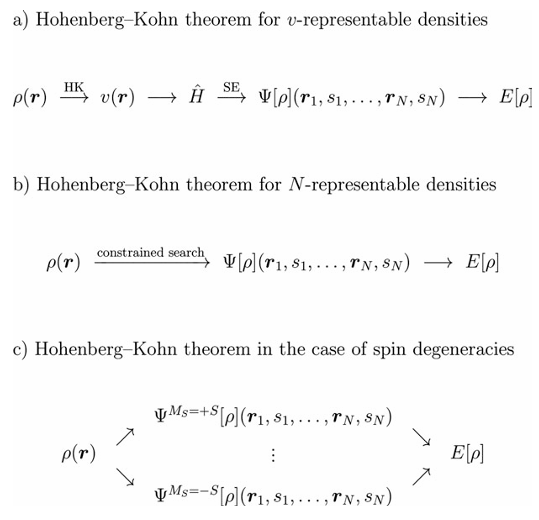
\includegraphics[width=0.6\linewidth]{image.png}
    \caption{Connection between the electron density \( \rho(\mathbf{r})\) and the total
 energy as stated by the first HK theorem.}
    \label{fig:enter-label}
\end{figure}



Connection between the electron density \( \rho(\mathbf{r})\) and the total
 energy as stated by the first HK theorem.


Thus, there is an energy functional \( E[\rho] \) that connects the electron density to the total energy. According to the second Hohenberg-Kohn (HK) theorem, the ground state energy \( E_0 \) of a system of electrons in a given nuclear potential \( v_{\text{nuc}}(r) \) can be found by minimizing the total energy functional.
\begin{equation}
     E_0 = \min_\rho E[\rho] 
\end{equation}
With

 \begin{equation}
     E[\rho] = q_e \int \rho(\mathbf{r}) v_{\text{nuc}}(\mathbf{r}) \, d^3r + F_{\text{HK}}[\rho] 
 \end{equation}


Under the constraint that \( \rho(\mathbf{r}) \) integrates to \( N \) electrons, the electron density that minimizes the energy functional is the ground-state electron density \( \rho_0(\mathbf{r}) \). The total energy functional is divided into a system-specific part (dependent on the nuclear potential) and a system-independent part, known as the "universal HK functional" \( F_{\text{HK}}[\rho] \). According to the Levy constrained-search formulation of DFT, this universal HK functional is defined as:


\begin{equation}
    F_{\text{HK}}[\rho] = \min_{\Psi \to \rho} \langle \Psi | \hat{T} + \hat{V}_{ee} | \Psi \rangle
\end{equation}



The operators \( \hat{T} \) and \( \hat{V}_{ee} \) represent the kinetic and electron-electron repulsion energies. Minimizing these over all wavefunctions \( \Psi \) that yield the target electron density \( \rho \) gives the exact ground-state density \( \rho_0 \) and wavefunction \( \Psi_0 \). This wavefunction must be an eigenfunction of \(\mathbf{ \hat{S}^2 }\).

The Levy-constrained search extends the domain from v-representable to N-representable densities, generalizing the first HK theorem. Degenerate states with \( S > 0 \) share the same electron density, and minimizing the total energy functional \( E[\rho] \) still leads to a unique ground-state density \( \rho_0 \). If a unique wavefunction is needed, the search can be restricted to wavefunctions with a specific \( M_S \) value.




\begin{itemize}
    \item \textbf{ Spin density in Hohenberg–Kohn DFT}
\end{itemize}




In density-functional theory (DFT), the \textbf{spin density} \( Q^{M_S}(\mathbf{r}) = \rho_\alpha^{M_S}(\mathbf{r}) - \rho_\beta^{M_S}(\mathbf{r}) \), representing the local excess of \( \alpha \)-spin electrons over \( \beta \)-spin electrons, is introduced to extend the Hohenberg-Kohn (HK) framework to spin-dependent systems. While the original HK theorems require only the total electron density \( \rho(r) \) to determine the ground-state energy, fixing a specific spin projection \( M_S \) allows the determination of both \( \rho(\mathbf{r}) \) and \( Q(\mathbf{r}) \) through the minimization of a generalized total energy functional \( E[\rho^\alpha, \rho^{\beta}] \). This functional is expressed as:

\begin{equation}
   E[\rho^\alpha, \rho^{\beta}] = q_e \int [\mathbf{\rho}^{\alpha}(\mathbf{r}) +\mathbf{\rho}^{\beta}(\mathbf{r})] v_{nuc}(\mathbf{r}) d^3r + F_{HK}[\mathbf{\rho}^{\alpha}, \mathbf{\rho}^{\beta}]
\end{equation}

where \( F_{HK}[\rho^\alpha, \rho^\beta] \) is the universal HK functional in terms of both the total electron density \( Q^{M_S[\rho]} \) and the spin density \( Q_0(\mathbf{r}) \). The functional \( F_{HK}[q, Q] \) is defined as:


\begin{equation}
    F_{HK}[\rho^{\alpha}, \rho^{\beta}] = \min_{\Psi \to \rho^{\alpha},  \rho^{\beta}} \langle \Psi | T + V_{ee} | \Psi \rangle
\end{equation},


where \( T \) is the kinetic energy operator and \( V_{ee} \) represents electron-electron interactions. The minimization is subject to the constraint that \( Q^{M_S}(\rho) \) integrates to \( M_S \):

\begin{equation}
    \frac{1}{2} \int Q^{M_S}(\mathbf{r}) \, d^3r = M_S.
\end{equation}
The individual spin densities \( \rho_\alpha(\mathbf{r}) \) and \( \rho_\beta(\mathbf{r}) \) can be calculated from the ground-state wavefunction \( \Psi^{M_S}[\rho] \) as:


\begin{equation}
    \rho_\alpha^{M_S}[\rho](\mathbf{r}) = N \int |\Psi^{M_S}[\rho](r, +1/2, \mathbf{r_2},s_2,...)|^2 \ d^3r_2 ds_2\cdots d^3r_N ds_N,
\end{equation}

\begin{equation}
    \rho_\beta^{M_S}[\rho](\mathbf{r}) = N \int |\Psi^{M_S}[\rho](r, -1/2, \mathbf{r_2},s_2,...)|^2 \ d^3r_2 ds_2\cdots d^3r_N ds_N,
\end{equation}

The spin density \( Q^{M_S}[\rho](\mathbf{r}) \) is then given by:

\begin{equation}
    Q^{M_S}[\rho](\mathbf{r}) = \rho_\alpha^{M_S}[\rho](\mathbf{r}) - \rho_\beta^{M_S}[\rho](\mathbf{r}).
\end{equation}

Minimizing \( F_{HK}[\rho, Q] \) with respect to \( Q(r) \), while enforcing the constraint on \( M_S \), ensures that the spin density \( Q(r) \) corresponds to the selected spin state. This generalization is crucial for describing open-shell systems such as radicals or magnetic materials. However, current approximate functionals often fail to satisfy exact properties, like maintaining constant energy for fractional spin densities, leading to errors in practical applications. 




\begin{itemize}
    \item \textbf{ Fractional spinconditionsontheHKfunctional
}
\end{itemize}

The Fractional Spin Conditions on the Hohenberg–Kohn Functional section addresses a key property of the exact spin-dependent HK functional, \( F_{HK}[\rho, Q] \), under conditions where the spin density \( Q(r) \) is fractional. Fractional spin densities arise when the spin state of a system is described as a linear combination or ensemble of spin states with specific \( M_S \) values. For example, consider a mixture of \( M_S = +S \) and \( M_S = -S \) states. In such cases, the spin density is given by:


\begin{equation}
    Q(r) = \alpha Q_{M_S=S}[\rho](r) + (1 - \alpha) Q_{M_S=-S}[\rho](r)
\end{equation},


where \( -1 \leq \alpha \leq 1 \). Importantly, for the exact HK functional, the energy functional must remain constant for any such linear combination:

\begin{equation}
    F_{HK}[\rho, \alpha Q^{M_S=S}[\rho]] = \text{const.}, \quad \text{for } -1 \leq \alpha \leq 1.
\end{equation}

This means that the functional \( F_{HK}[\rho, \alpha Q^{M_S=S}[\rho]\) is invariant with respect to fractional spin densities derived from ensemble mixtures of spin states.

\textbf{Key Insights:}\\
1.\textbf{ Degeneracy and Fractional Spin:}\\
 For systems with spin \( S > 0 \), the wavefunctions \( \Psi_{M_S} \) corresponding to different \( M_S \) values are degenerate and produce distinct spin densities \( Q^{M_S}[\rho](\alpha) \). These densities are scaled versions of the highest \( M_S \) spin density:
   \begin{equation}
        Q^{M_S}[\rho](\mathbf{r}) = \frac{M_S}{S} Q^{M_S=S}[\rho](\mathbf{r})
   \end{equation}
     leading to \( Q_{M_S=-S}(r) = -Q_{M_S=S}(r) \) and \( Q_{M_S=0}(r) = 0 \) for even \( S \).\\
    
\textbf{
2. Ensemble Spin Densities:}\\
    Linear combinations of spin densities form "fractional spins." For such fractional densities, the exact total energy functional \( E[\rho, Q] \) must yield the same energy:
     \begin{equation}
         E[\rho, \alpha Q^{M_S=S}[\rho]] = \text{const.}, \quad \forall \alpha \in [-1, 1].
     \end{equation}
\textbf{
3. Implications for Approximate Functionals:}
   Current approximate exchange-correlation functionals \( E_{xc}[\rho, Q] \) fail to satisfy this constancy condition, introducing errors in practical calculations. These errors often manifest in systems with near-degenerate spin states, where the energy varies incorrectly with fractional spins.\\

\textbf{4. Relation to Spin-Independent Functionals:}
   - The constancy condition simplifies the relationship between the spin-independent and spin-dependent HK functionals. Specifically, the spin-independent functional \( F_{HK}[\rho] \) corresponds to the spin-dependent functional evaluated at \( Q(\mathbf{r}) = 0 \):
   
     \begin{equation}
          F_{HK}[\rho] = F_{HK}[\rho, Q = 0]
     \end{equation}

This section highlights the fundamental nature of fractional spin conditions in exact DFT and emphasizes the limitations of current approximations. Addressing these limitations is crucial for improving the accuracy of DFT for systems with complex spin states or fractional spin behavior. 




\begin{itemize}
    \item \textbf{Spin States in Hohenberg–Kohn DFT}
\end{itemize}

This section discusses how the Hohenberg–Kohn (HK) theorems can be generalized to include the lowest-energy states of a given spin symmetry. While the original HK theorems are only applicable to the ground state, this generalization allows the calculation of the lowest-energy state with a specific spin \( S \) by modifying the functional framework.

\textbf{ Spin-Specific Energy Functional}

To determine the lowest-energy state with a specific value of the total spin \( S \), a spin-state specific energy functional is defined as:

\begin{equation}
    E^S[\rho] = q_e \int \rho(\mathbf{r}) v_{\text{nuc}}(\rho) d^3r + F_{HK}^{S}[\rho]
\end{equation}
where \( F_{HK}^{S}[\rho] \) is the spin-state specific HK functional given by:
\begin{equation}
    F_{HK}^{S}[\rho] = \min_{\Psi^S \to \rho} \langle \Psi^S | T + V_{ee} | \Psi^S \rangle
\end{equation}

subject to the constraint that \( \Psi^S \) is an eigenfunction of the total spin operator \( \hat{S}^2 \) with eigenvalue \( S(S + 1)\hbar^2 \). This constraint ensures that the wavefunction belongs to a specific spin state. Therefore, different spin states \( S \) lead to distinct HK functionals and total energy functionals.

Use of \( M_S \) to Approximate Spin Selection

In practice, spin-DFT often uses the spin projection quantum number \( M_S \) to approximate spin selection. By fixing \( M_S \), the minimization of the total energy functional \( E[\rho, Q] \) is constrained to states with \( S \geq M_S \). The corresponding spin-state energy is:

\begin{equation}
    E^{S \geq M_S}[\rho] = E[\rho, Q^{M_S}[\rho]]
\end{equation}

where \( Q^{M_S}[\rho] \) is the spin density associated with the chosen value of \( M_S \). The minimization ensures that:


\begin{equation}
    \frac{1}{2} \int Q_{M_S}(r) d^3r = M_S.
\end{equation}


This method effectively selects the lowest-energy state for \( S \geq M_S \). However, this approach is not entirely general. For instance, while it can target the lowest triplet (\( S = 1 \)) state when the ground state is a singlet (\( S = 0 \)), it cannot target the lowest singlet state if the ground state is a triplet.

 Challenges in Targeting Specific Spin States

To rigorously compute the lowest-energy state for a specific \( S \), the full spin-state specific energy functional \( E_S[\rho] \) is required. While using \( M_S \) provides a practical approximation, it lacks the ability to fully isolate states of a specific \( S \). This limitation is particularly important when spin states of different \( S \) values are close in energy, as in many open-shell systems or transition metal complexes.





\section{Spin in Kohn–Sham DFT}

The Hohenberg-Kohn formulation discussed in the previous section, while exact, is not computationally practical to implement. This difficulty arises primarily from the challenge of expressing the kinetic energy in the HK functional directly as a functional of the electron density. To address this issue in practical applications of DFT, Kohn and Sham proposed an alternative approach. They introduced a reference system of non-interacting electrons that reproduces the same electron density as the original interacting system. The kinetic energy of this reference system closely approximates that of the interacting system, with only a small residual term that must be approximated.\\

The relationship between the original system and the reference system is illustrated in Fig.\ref{fig:KS-DFT}. In this context, the system of noninteracting electrons is divided into two categories: a spin-restricted reference system and a spin-unrestricted reference system. For all three systems under consideration, the electron density $\rho(\mathbf{r})$ remains the same, as it is independent of whether electron interactions are present or absent. However, the wavefunctions $\Psi(\mathbf{x}_1,...,\mathbf{x}_N)$ and spin densities $Q(\mathbf{r})$  are not necessarily identical across the systems. This discrepancy arises due to the electron-electron interaction contribution in the Hamiltonian of the original system. Specifically,
\begin{equation}
    \rho(\mathbf{r}) =\rho_s^{(u)}(\mathbf{r})=\rho_s(\mathbf{r}),
\end{equation}
\begin{equation}
    \Psi(\mathbf{x}_1,...,\mathbf{x}_N) \neq \Psi_s^{(u)}(\mathbf{x}_1,...,\mathbf{x}_N) \neq \Psi_s(\mathbf{x}_1,...,\mathbf{x}_N),
    \label{eq:65}
\end{equation}
\begin{equation}
    Q(\mathbf{r}) = Q_s^{(u)}(\mathbf{r}) \neq Q_s(\mathbf{r}).
    \label{eq:66}
\end{equation}

The subscript $s$ refers to the spin-restricted reference system, while the superscript $(u)$ combined with the subscript $s$ represents the spin-unrestricted reference system. The specific details of the relationships in Eqs.~\eqref{eq:65} and \eqref{eq:66}, as well as the characteristics of the Kohn-Sham DFT formalism for both spin-restricted and spin-unrestricted reference systems, will be discussed in the following subsections.\\

\begin{figure}[ht]
    \centering
    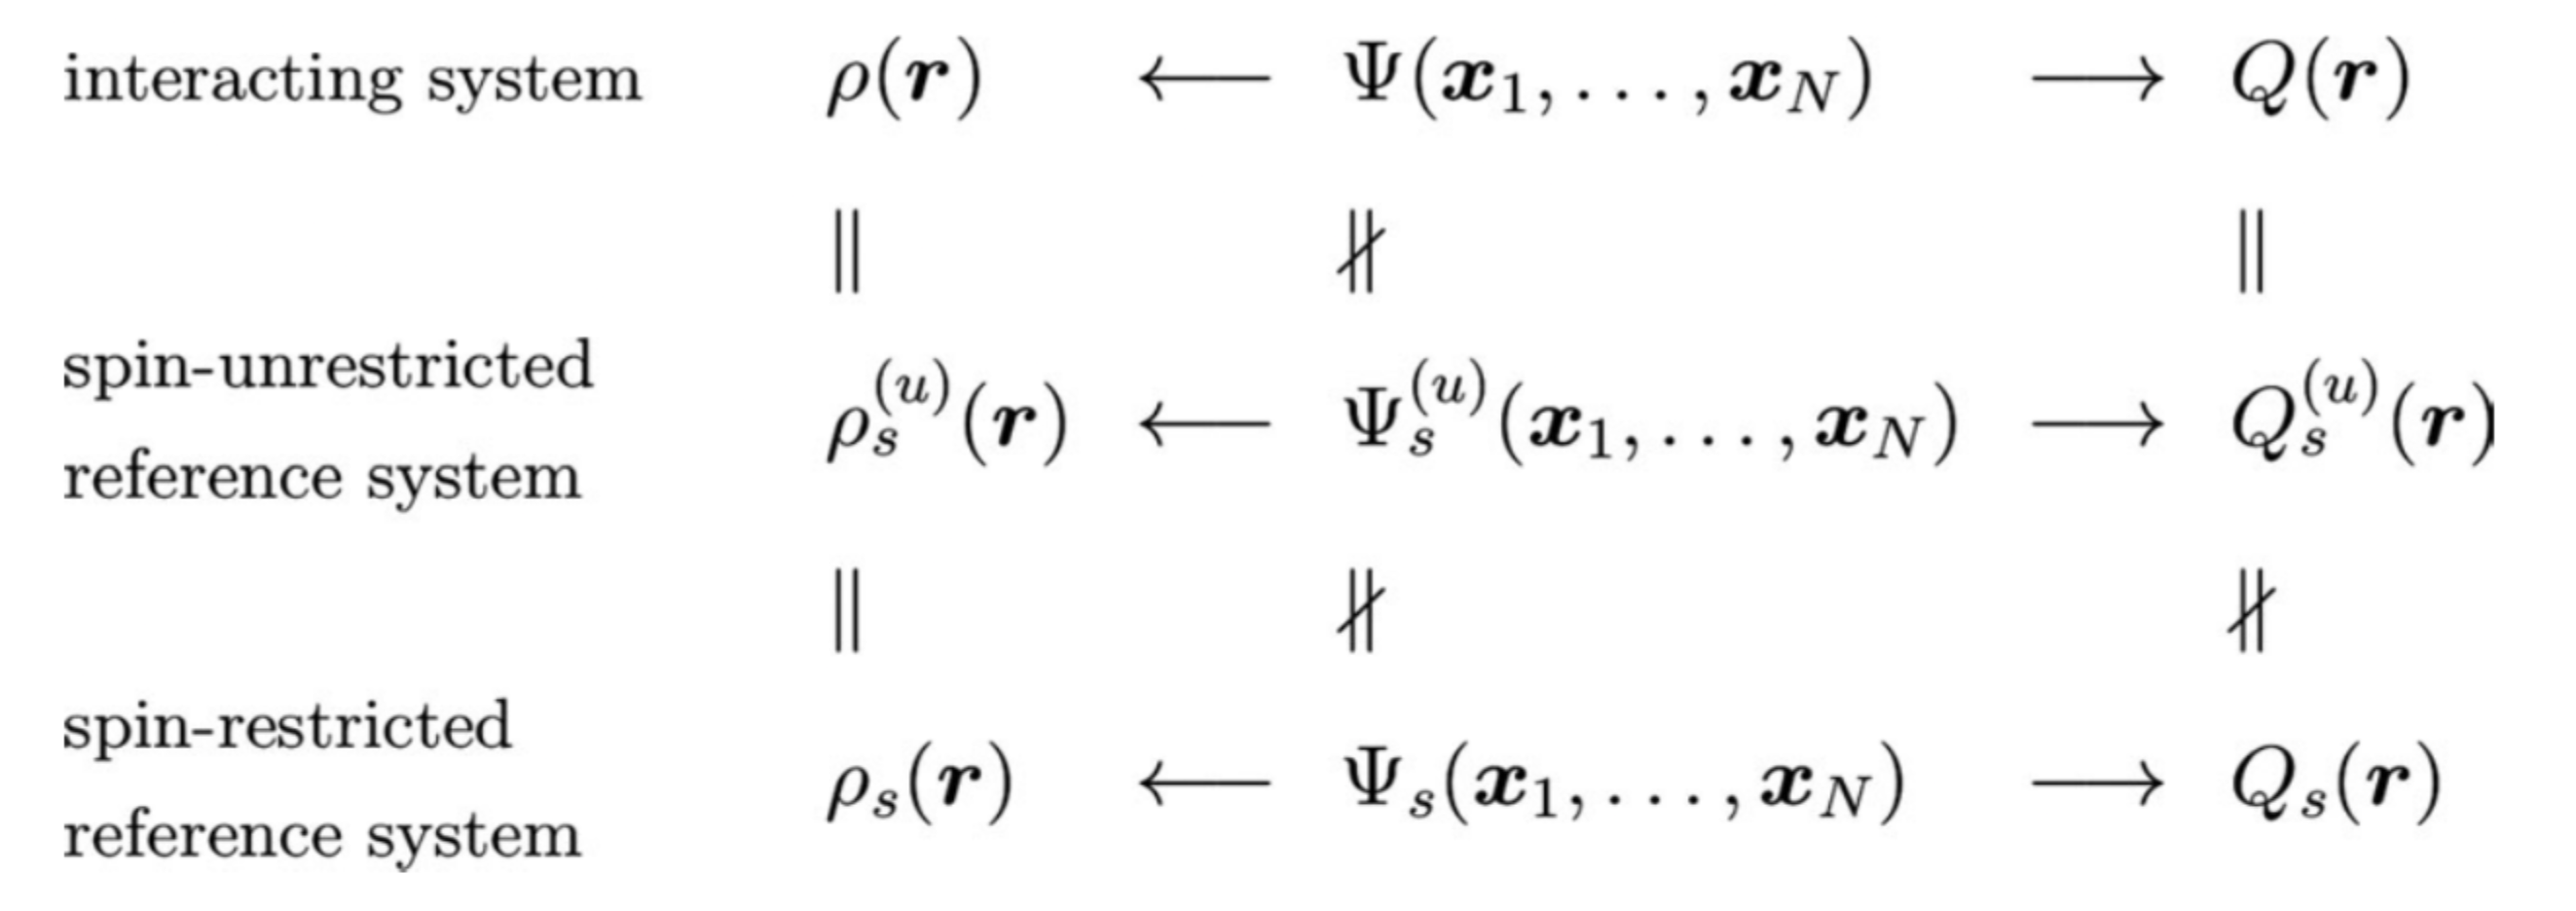
\includegraphics[width=0.8\linewidth]{Spin KS-DFT.png}
    \caption[Illustration of the connection between the interacting electron system and the non-interacting reference system in Kohn-Sham density functional theory.]{Illustration of the connection between the interacting electron system and the non-interacting reference system in Kohn-Sham density functional theory. The reference system is further categorized into spin-restricted and spin-unrestricted cases.}
    \label{fig:KS-DFT}
\end{figure}

\begin{itemize}
    \item  \textbf{Spin-Restricted Kohn–Sham DFT}
\end{itemize}

This section describes how the Kohn–Sham (KS) formulation of DFT can be applied to systems with spin restrictions. In spin-restricted Kohn–Sham DFT, the total electron density \( \rho(\mathbf{r}) \) is treated as the sum of contributions from spin-up (\( \alpha \)) and spin-down (\( \beta \)) electrons, but the spatial distribution of these electrons is constrained to be identical. This results in a simpler framework, particularly for closed-shell systems.

Noninteracting Reference System

The KS approach introduces a noninteracting reference system of electrons described by the Hamiltonian:


\begin{equation}
    \hat{H}_s = \hat{T} + \hat{V}_s = \sum_{i=1}^N \left( -\frac{\hbar^2}{2m_e} \nabla_i^2 + q_e v_s(\mathbf{r_i}) \right)
\end{equation}


where \( v_s(\mathbf{r}) \) is the effective single-particle potential. Since this Hamiltonian does not couple different electrons, the exact wavefunction of the noninteracting system can be written as a single Slater determinant:


\begin{equation}
    \Psi_s(x_1, \dots, x_N) = |\phi_1 \alpha,\phi_1\beta,\phi_2\alpha\phi_2\beta|
\end{equation}


where the \( \Phi_i(x) \) are one-electron spin orbitals. These orbitals are solutions to the KS equations:

\begin{equation}
    \left( -\frac{\hbar^2}{2m_e} \nabla^2+ q_e v_s(\mathbf{r}) \right) \phi_i(\mathbf{r}) = \epsilon_i \phi_i(\mathbf{r})
\end{equation}
where \( \epsilon_i \) are the orbital energies.

 Total Electron Density and Spin Density

In a spin-restricted formulation, each spatial orbital \( \phi_i(\mathbf{r}) \) can either be doubly occupied (one \( \alpha \) and one \( \beta \) electron) or singly occupied. The total electron density is given by:

\begin{equation}
    \rho(\mathbf{r}) = \sum_i^{\text{occ. } } f_i |\phi_i(\mathbf{r})|^2
\end{equation}

where \( f_i \) represents the occupation number of the orbital, taking values \( f_i = 2 \) for doubly occupied orbitals and \( f_i = 1 \) for singly occupied orbitals.

Since the spatial parts of the orbitals for \( \alpha \) and \( \beta \) electrons are identical in the spin-restricted case, the spin density \( Q_s(\mathbf{r}) \) depends only on the singly occupied orbitals:

\begin{equation}
    Q_s(r) = \sum_i^{\text{singly occ. } } s_i |\phi_i(\mathbf{r})|^2
\end{equation}

Where \( s_i = +1 \) for \( \alpha \)-spin electrons and \( s_i = -1 \) for \( \beta \)-spin electrons.

 Kinetic Energy of the Non-interacting System

The kinetic energy of the spin-restricted system is given by:


\begin{equation}
    T_s = \sum_i^{\text{occ. }} f_i \langle \phi_i | \hat{T} | \phi_i \rangle = -\frac{\hbar^2}{2m_e} \sum_i^{\text{occ. } } f_i \int \phi_i(\mathbf{r}) \nabla \phi_i(\mathbf{r}) \, d^3r
\end{equation}


 Energy Functional

The total energy of the interacting system is expressed as:

\begin{equation}
    E[q] = T_s[\rho] + J[\rho] + E_{xc}[\rho,Q] + q_e \int \rho(\mathbf{r}) v_{\text{nuc}}(\mathbf{r}) \, d^3r
\end{equation}


Where:
\( T_s[\rho] \): Noninteracting kinetic energy.
 \( J[\rho] \): Classical Coulomb repulsion energy:
  \begin{equation}
        J[\rho] = \frac{q_e^2}{2} \int \frac{\rho(\mathbf{r}) \rho(\mathbf{r'})}{\mathbf{|r - r'}|} \, d^3r \, d^3r'.
  \end{equation}
\( E_{xc}[\rho] \): Exchange-correlation energy functional.

\textbf{Kohn–Sham Potential}

Minimizing the total energy functional with respect to \( \rho(r) \) yields the effective KS potential:

\begin{equation}
    v_s[\rho](\mathbf{r}) = v_{\text{nuc}}(\mathbf{r}) + v_{\text{Coul}}[\rho](\mathbf{r}) + v_{xc}[\rho](\mathbf{r})
\end{equation}

where:
 \( v_{\text{Coul}}[\rho](\mathbf{r}) \): Classical Coulomb potential:
  \[
  v_{\text{Coul}}[\rho](\mathbf{r}) = q_e \int \frac{\rho(r')}{|r - r'|} \, d^3r'.
  \]
 \( v_{xc}[\rho](\mathbf{r}) \): Exchange correlation potential:
  \begin{equation}
      v_{xc}[\rho](\mathbf{r}) = \frac{1}{q_e} \frac{\delta E_{xc}[\rho]}{\delta \rho(\mathbf{r})}.
  \end{equation}

 Summary of Spin-Restricted KS-DFT

In spin-restricted KS-DFT, the total density \( \rho(\mathbf{r}) \) is identical for \( \alpha \)- and \( \beta \)-spin electrons, simplifying the treatment of closed-shell systems. This approach assumes that the noninteracting reference system has the same electron density as the true interacting system, even though their wavefunctions and spin densities may differ. This constraint results in a framework that is computationally efficient and well-suited for closed-shell molecules but less accurate for open-shell systems where spin polarization is significant.


\begin{itemize}
    \item  \textbf{Spin-Unrestricted Kohn–Sham DFT}
\end{itemize}

Unlike the spin-restricted reference system, it is possible to define a reference system of noninteracting electrons that replicates the same $\alpha$ and $\beta$ electron densities as the original interacting system. For this purpose, a reference system governed by the Hamiltonian
\begin{align}
    \hat{H}_s^{(u)} &= \hat{T}_s + \hat{V}_s^{tot} + \hat{V}_s^{spin} = \sum_{i=1}^{N}\frac{\hbar^2}{2m_e}\nabla_i^2 + q_e\sum_{i=1}^{N}\left[ v_s^{tot}(\mathbf{r}_i) + v_s^{spin}(\mathbf{r}_i)\sigma_z(s_i) \right], \\
   \hat{H}_s^{(u)} &= \hat{T}_s + \hat{V}_s^{\alpha} + \hat{V}_s^{\beta} = \sum_{i=1}^{N}\frac{\hbar^2}{2m_e}\nabla_i^2 + q_e\sum_{i=1}^{N}\left[ v_s^{\alpha}(\mathbf{r}_i)\alpha(s_i) - v_s^{\beta}(\mathbf{r}_i)\beta(s_i) \right],
    \label{eq:78}
\end{align}
is employed. In this setup, distinct potentials $v_s^{\alpha}(\mathbf{r}_i) = v_s^{tot}(\mathbf{r}_i) + v_s^{spin}(\mathbf{r}_i)$ and $v_s^{\beta}(\mathbf{r}_i) = v_s^{tot}(\mathbf{r}_i) - v_s^{spin}(\mathbf{r}_i)$ are required for $\alpha$ and $\beta$ electrons, respectively. These potentials ensure that the reference system of noninteracting electrons reproduces the same spin density as the interacting system. This is equivalent to introducing an inhomogeneous external magnetic field in the $z$-direction, $B_z(\mathbf{r}) = -\frac{q_e}{\mu_B}v_s^{spin}(\mathbf{r})$, which interacts solely with the electronic spins.\\

The exact solution to the corresponding Schrödinger equation is represented by a single Slater determinant. However, unlike the spin-restricted case, the spatial orbitals for $\alpha$ and $\beta$ electrons differ, such that
\begin{equation}
    \Psi_s(\mathbf{x}_1, \dots, \mathbf{x}_N) = |\phi_1^{\alpha} \alpha,\phi_1^{\beta}\beta,\phi_2^{\alpha}\alpha,\phi_2^{\beta}\beta,...|.
\end{equation}

The spatial components of these orbitals are determined through two distinct sets of one-electron equations:
\begin{align}
    \left[ -\frac{\hbar^2}{2m_e}\nabla^2 + q_ev_s^{\alpha}(\mathbf{r}) \right]\phi_i^{\alpha}(\mathbf{r}) &= \epsilon_i^{\alpha}\phi_i^{\alpha}(\mathbf{r}), \\
    \left[ -\frac{\hbar^2}{2m_e}\nabla^2 + q_ev_s^{\beta}(\mathbf{r}) \right]\phi_i^{\beta}(\mathbf{r}) &= \epsilon_i^{\beta}\phi_i^{\beta}(\mathbf{r}).
\end{align}

The resulting $\alpha$ and $\beta$ orbitals each form an orthonormal set. However, $\alpha$ and $\beta$ orbitals are generally not orthogonal to one another.\\

The noninteracting Hamiltonian $\hat{H}_s^{(u)}$ retains its commutation relationship with the spin projection operator $\hat{S}_z$. Consequently, any spin-unrestricted Slater determinant remains an eigenfunction of $\hat{S}_z$, with its eigenvalue $M_S$ determined by the difference in the number of $\alpha$ and $\beta$ electrons. However, unlike in the spin-restricted case, the eigenstates of $\hat{S}_z$ are no longer degenerate, as the energies of orbitals for $\alpha$ and $\beta$ electrons differ due to the spin-dependent potentials.\\

To construct the ground-state wavefunction in this framework, the $N$ orbitals with the lowest orbital energies must be filled, and this process inherently determines the value of $M_S$. Once these lowest-energy orbitals are occupied, the system achieves the configuration that minimizes the energy for the reference system. On the other hand, excited-state wavefunctions for the noninteracting reference system can be generated by occupying higher-energy orbitals. This approach also allows for the exploration of configurations with different $M_S$ values, as the distribution of $\alpha$ and $\beta$ electrons among the orbitals can be adjusted. Thus, spin-unrestricted systems offer a broader range of configurations compared to spin-restricted systems, making them particularly useful for studying systems where spin polarization plays a significant role.\\

The unrestricted Hamiltonian $\hat{H}_s^{(u)}$ generally does not commute with the total spin operator $\hat{\mathbf{S}}^2$ meaning that the ground-state wavefunction of the system is not guaranteed to be an eigenfunction of $\hat{\mathbf{S}}^2$. Instead of having a well-defined spin quantum number, the ground-state spin properties are described through the expectation value of $\hat{\mathbf{S}}^2$, which can be computed as
\begin{equation}
    \left\langle  \hat{\mathbf{S}}^2 \right\rangle = M_S(M_S+1)\hbar^2 + \hbar^2N_{\beta} - \hbar^2\sum_{i=1}^{N_{\alpha}}\sum_{i=1}^{N_{\beta}}\left| \int\phi_i^{\alpha}(\mathbf{r})\phi_i^{\beta}(\mathbf{r})\mathrm{d}^3r \right|^2.
\end{equation}

Here, the last term captures the overlap between spatial orbitals for $\alpha$ and $\beta$ electrons. In the spin-restricted formalism, $\alpha$ and $\beta$ orbitals are identical and orthogonal, which simplifies the overlap term to equal the number of doubly occupied orbitals. As a result, the expectation value reduces to $\left\langle  \hat{\mathbf{S}}^2 \right\rangle = M_S(M_S+1)\hbar^2$. However, in the spin-unrestricted case, $\alpha$ and $\beta$ orbitals differ spatially and are not necessarily orthogonal. This partial overlap leads to an additional contribution in the expectation value of $\hat{\mathbf{S}}^2$, resulting in a larger value than the ideal $M_S(M_S+1)\hbar^2$. This deviation, termed 'spin contamination', reflects the mixing of states with higher spin multiplicities into the ground-state wavefunction.\\

Spin contamination is a significant limitation of the unrestricted approach, especially in systems with strong electron correlation or open-shell configurations. It can lead to inaccuracies in the predicted energies and properties of the system. Correcting spin contamination often requires advanced post-Hartree-Fock methods or spin projection techniques.\\

For an unrestricted Slater determinant, the total electron density is given by
\begin{equation}
    \rho(\mathbf{r}) = \sum_{i=1}^{N_{\alpha}}|\phi_i^{\alpha}(\mathbf{r})|^2 + \sum_{i=1}^{N_{\beta}}|\phi_i^{\beta}(\mathbf{r})|^2,
\end{equation}
and the spin density can be calculated as
\begin{equation}
    Q(\mathbf{r}) = \sum_{i=1}^{N_{\alpha}}|\phi_i^{\alpha}(\mathbf{r})|^2 - \sum_{i=1}^{N_{\beta}}|\phi_i^{\beta}(\mathbf{r})|^2.
\end{equation}

The kinetic energy of the unrestricted Slater determinant $\Psi_s^{(u)}$ is
\begin{align}
    T_s^{(u)} &= \bra{\Psi_s}\hat{T}\ket{\Psi}, \\
    &= -\frac{\hbar^2}{2m_e}\left[ \sum_{i=1}^{N_{\alpha}}\int\phi_i^{\alpha}\nabla^2\phi_i^{\alpha}\mathrm{d}^3r + \sum_{i=1}^{N_{\beta}}\int\phi_i^{\beta}\nabla^2\phi_i^{\beta}\mathrm{d}^3r \right],
\end{align}
and a noninteracting kinetic energy functional can now be defined as
\begin{equation}
    T_s^{(u)}[\rho_{\alpha},\rho_{\beta}] = \text{min}_{\Psi_s^{(u)}\to \rho_{\alpha},\rho_{\beta}}\bra{\Psi_s^{(u)}}\hat{T}\ket{\Psi_s^{(u)}},
\end{equation}
or as
\begin{equation}
    T_s^{(u)}[\rho, Q] = \text{min}_{\Psi_s^{(u)}\to \rho,Q}\bra{\Psi_s^{(u)}}\hat{T}\ket{\Psi_s^{(u)}}.
\end{equation}

In terms of $\alpha$ and $\beta$ electron densities, the total energy functional of the noninteracting system is given by
\begin{equation}
    E_s^{(u)}[\rho_{\alpha},\rho_{\beta}] = T_s^{(u)}[\rho_{\alpha},\rho_{\beta}] + q_e\left[ \int\rho_{\alpha}(\mathbf{r})v_s^{\alpha}(\mathbf{r})\mathrm{d}^3r + \int\rho_{\beta}(\mathbf{r})v_s^{\beta}(\mathbf{r})\mathrm{d}^3r \right].
\end{equation}

The ground-state $\alpha$ and $\beta$ densities $\rho_0^{\alpha}(\mathbf{r})$ and $\rho_0^{\beta}(\mathbf{r})$ can then be determined by minimizing this energy functional with respect to $\rho_{\alpha}$ and $\rho_{\beta}$, under the constraint that these integrate to the correct number of $\alpha$ and $\beta$ electrons.\\

The spin-resolved HK functional of the original interacting system can now be written as
\begin{equation}
    F_{KH}[\rho_{\alpha},\rho_{\beta}] = T_s^{(u)}[\rho_{\alpha},\rho_{\beta}] + J[\rho] + E_{xc}^{(u)}[\rho_{\alpha},\rho_{\beta}],
\end{equation}
where the spin-resolved exchange-correlation energy is defined as
\begin{equation}
    E_{xc}^{(u)}[\rho_{\alpha},\rho_{\beta}] = F_{KH}[\rho_{\alpha},\rho_{\beta}] - T_s^{(u)}[\rho_{\alpha},\rho_{\beta}] - J[\rho].
\end{equation}

With this definition of the exchange-correlation energy, the total energy functional of the original interacting system is given by
\begin{equation}
    E[\rho_{\alpha},\rho_{\beta}] = T_s^{(u)}[\rho_{\alpha},\rho_{\beta}] + J[\rho] + E_{xc}^{(u)}[\rho_{\alpha},\rho_{\beta}] + q_e\int\rho(\mathbf{r})v_{nuc}(\mathbf{r})\mathrm{d}^3r.
\end{equation}

The ground-state $\alpha$ and $\beta$ electron densities $\rho_0^{\alpha}(\mathbf{r})$ and $\rho_0^{\beta}(\mathbf{r})$ can then be determined by minimizing this total energy functional with respect to $\rho_{\alpha}$ and $\rho_{\beta}$, under the constraint that these integrate to $N_{\alpha}$ and $N_{\beta}$ electrons, respectively.\\

The minimization of the total energy functional $E[\rho_{\alpha},\rho_{\beta}]$ of the spin-unrestricted noninteracting reference system leads to these Euler-Lagrange equations
\begin{align}
    \frac{\delta E_s^{(u)}[\rho_{\alpha},\rho_{\beta}]}{\delta\rho_{\alpha}(\mathbf{r})} - \mu_{\alpha} &= \frac{\delta T_s^{(u)}[\rho_{\alpha},\rho_{\beta}]}{\delta\rho_{\alpha}(\mathbf{r})} + q_ev_s^{\alpha}(\mathbf{r}) - \mu_{\alpha} = 0, \\
    \frac{\delta E_s^{(u)}[\rho_{\alpha},\rho_{\beta}]}{\delta\rho_{\beta}(\mathbf{r})} - \mu_{\beta} &= \frac{\delta T_s^{(u)}[\rho_{\alpha},\rho_{\beta}]}{\delta\rho_{\beta}(\mathbf{r})} + q_ev_s^{\beta}(\mathbf{r}) - \mu_{\beta} = 0.
\end{align}

For the interacting system, the minimization of $E[\rho_{\alpha},\rho_{\beta}]$ with respect to the $\alpha$ and $\beta$ electron densities yields
\begin{align}
    \frac{\delta E_s^{(u)}[\rho_{\alpha},\rho_{\beta}]}{\delta\rho_{\alpha}(\mathbf{r})} - \mu_{\alpha} &= \frac{\delta T_s^{(u)}[\rho_{\alpha},\rho_{\beta}]}{\delta\rho_{\alpha}(\mathbf{r})} + q_e(v_{nuc}(\mathbf{r}) + v_{Coul}[\rho](\mathbf{r}) + v_{xc}^{\alpha}[\rho_{\alpha},\rho_{\beta}](\mathbf{r})) - \mu_{\alpha} = 0, \\
    \frac{\delta E_s^{(u)}[\rho_{\alpha},\rho_{\beta}]}{\delta\rho_{\beta}(\mathbf{r})} - \mu_{\beta} &= \frac{\delta T_s^{(u)}[\rho_{\alpha},\rho_{\beta}]}{\delta\rho_{\beta}(\mathbf{r})} + q_e(v_{nuc}(\mathbf{r}) + v_{Coul}[\rho](\mathbf{r}) + v_{xc}^{\beta}[\rho_{\alpha},\rho_{\beta}](\mathbf{r})) - \mu_{\beta} = 0,
\end{align}
with the spin components of the exchange-correlation potential
\begin{align}
    v_{xc}^{\alpha}[\rho_{\alpha},\rho_{\beta}](\mathbf{r}) &= \frac{1}{q_e} \frac{\delta E_{xc}^{(u)}[\rho_{\alpha},\rho_{\beta}]}{\delta\rho_{\alpha}(\mathbf{r})}, \\
    v_{xc}^{\beta}[\rho_{\alpha},\rho_{\beta}](\mathbf{r}) &= \frac{1}{q_e} \frac{\delta E_{xc}^{(u)}[\rho_{\alpha},\rho_{\beta}]}{\delta\rho_{\beta}(\mathbf{r})}.
\end{align}

If we require that $\rho_{\alpha}(\mathbf{r})$ and $\rho_{\beta}(\mathbf{r})$ are the same for the noninteracting reference system and the original interacting system, we find that the spin components of the KS potential are given by
\begin{align}
    v_s^{\alpha}[\rho_{\alpha},\rho_{\beta}](\mathbf{r}) &= v_{ext}(\mathbf{r}) + v_{Coul}[\rho](\mathbf{r}) + v_{xc}^{\alpha}[\rho_{\alpha},\rho_{\beta}](\mathbf{r}), \\
    v_s^{\beta}[\rho_{\alpha},\rho_{\beta}](\mathbf{r}) &= v_{ext}(\mathbf{r}) + v_{Coul}[\rho](\mathbf{r}) + v_{xc}^{\beta}[\rho_{\alpha},\rho_{\beta}](\mathbf{r}).
\end{align}

Therefore, the exact ground-state $\alpha$ and $\beta$ electron densities of the original interacting system can be calculated by solving the Schrödinger equation of an auxiliary system of noninteracting electrons with the Hamiltonian of Eq.~\eqref{eq:78}. The ground-state wavefunction $\Psi_{s,0}^{(u)}$ of this KS reference system is given by an unrestricted Slater determinant, constructed from the orbitals obtained from the KS equations,
\begin{align}
    \left[ -\frac{\hbar^2}{2m_e}\nabla^2 + q_e(v_{nuc}(\mathbf{r}) + v_{Coul}[\rho](\mathbf{r}) + v_{xc}^{\alpha}[\rho_{\alpha},\rho_{\beta}](\mathbf{r})) \right]\phi_i^{\alpha}(\mathbf{r}) &= \epsilon_i^{\alpha}\phi_i^{\alpha}(\mathbf{r}), \\
    \left[ -\frac{\hbar^2}{2m_e}\nabla^2 + q_e(v_{nuc}(\mathbf{r}) + v_{Coul}[\rho](\mathbf{r}) + v_{xc}^{\beta}[\rho_{\alpha},\rho_{\beta}](\mathbf{r})) \right]\phi_i^{\beta}(\mathbf{r}) &= \epsilon_i^{\beta}\phi_i^{\beta}(\mathbf{r}).
\end{align}

Equivalently, the KS potential can be expressed as a component that acts on the total electron density
\begin{equation}
    v_s^{tot}[\rho, Q](\mathbf{r}) = v_{ext}(\mathbf{r}) + v_{Coul}[\rho](\mathbf{r}) + v_{xc}^{tot}[\rho,Q](\mathbf{r}),
\end{equation}
and one that acts on the spin density
\begin{equation}
    v_s^{spin}[\rho, Q](\mathbf{r}) = v_{xc}^{spin}[\rho, Q](\mathbf{r}),
\end{equation}
where the total and spin exchange-correlation potential are given by
\begin{equation}
    v_{xc}^{tot}[\rho, Q] = \frac{1}{q_e}\frac{\delta E_{xc}^{(u)}[\rho]}{\delta \rho(\mathbf{r})},
\end{equation}
and
\begin{equation}
    v_{xc}^{spin}[\rho, Q] = \frac{1}{q_e}\frac{\delta E_{xc}^{(u)}[\rho]}{\delta Q(\mathbf{r})}.
\end{equation}

\begin{itemize}
    \item \textbf{ Comparison of restricted and unrestricted
    formulation}
\end{itemize}
The Kohn-Sham Density Functional Theory (KS-DFT) can be formulated in two principal ways: the restricted formulation and the unrestricted formulation. The choice between these two approaches has significant implications for the description of open-shell systems. Below, the key distinctions between the two formulations are discussed, along with the relevant equations and theoretical concepts.

In the restricted formulation, the non-interacting reference system is defined such that its total electron density \(\rho_s(\mathbf{r})\) matches the total electron density of the fully interacting system. However, the spin density \(Q_s(\mathbf{r})\) of the reference system may differ from that of the interacting system. Conversely, in the unrestricted formulation, both the total electron density \(\rho_s(\mathbf{r})\) and the spin density \(Q_s(\mathbf{r})\) of the reference system match those of the fully interacting system. This distinction imposes a stricter definition for the spin density in the unrestricted case.

The wavefunction \(\Psi_s\) of the non-interacting reference system in the restricted formulation can be chosen as an eigenvector of the operator \(\hat{S}^2\). However, the eigenvalue \(\langle \hat{S}^2 \rangle = S(S+1) \hbar^2\) does not necessarily match that of the interacting system. This mismatch can be resolved by imposing an additional constraint on the system. In the unrestricted formulation, the wavefunction \(\Psi_s^{(u)}\) is generally not an eigenvector of \(\hat{S}^2\) for \(S > 0\), which is known as spin contamination. This contamination arises from the requirement to reproduce the correct spin density of the interacting system, making \(\langle \hat{S}^2 \rangle\) a more complex functional of the electron density.

In both formulations, the wavefunction of the reference system is an eigenvector of the operator \(\hat{S}_z\). However, in the unrestricted formulation, the corresponding eigenvalue \(M_S\) always matches that of the interacting system. In the restricted formulation, it is possible to select this value accordingly, but it is not guaranteed to be correct.

The kinetic energy of the non-interacting system is another critical aspect of these formulations. In the restricted formulation, the kinetic energy \(T_s^(u)[\rho, Q]\) is defined as the kinetic energy of a system of non-interacting electrons with total electron density \(\rho(\mathbf{r})\), and it does not depend on the spin density \(Q(r)\). In the unrestricted formulation, the kinetic energy \(T_s^{(u)}[\rho, Q]\) is defined as the kinetic energy of a system of non-interacting electrons with both total electron density \(\rho(\mathbf{r})\) and spin density \(Q(\mathbf{r})\). These kinetic energies differ by the term 
\begin{equation}
    T_u[\rho, Q] = T_s[\rho] - T_s^{(u)}[\rho, Q]
\end{equation}.
Only when the spin density is zero do the two definitions coincide.

The exchange-correlation energy is defined differently in the two formulations. In the restricted formulation, the exchange-correlation energy \(E_{xc}[\rho, Q]\) is expressed through the decomposition of the Hohenberg-Kohn (HK) functional as:
\begin{equation}
    F_{HK}[\rho, Q] = T_s[\rho] + J[\rho] + E_{xc}[\rho, Q]
\end{equation}
In the unrestricted formulation, the exchange-correlation energy \(E_{xc}^{(u)}[\rho, Q]\) is defined in terms of the non-interacting kinetic energy \(T_s^{(u)}[\rho, Q]\) as follows:
\begin{equation}
    F_{HK}[\rho, Q] = T_s^{(u)}[\rho, Q] + J[\rho] + E_{xc}^{(u)}[\rho, Q]
\end{equation}
These energies are related by the equation:
\begin{equation}
     E_{xc}^{(u)}[\rho, Q] = E_{xc}[\rho, Q] + T_u[\rho, Q]
\end{equation}
The exchange-correlation potential, which plays a key role in the Kohn-Sham equations, also differs in the two formulations. In the restricted formulation, the exchange-correlation potential \(v_{xc}[\rho]\) acts on the total electron density \(\rho( \mathbf{r})\) and is defined as:
\begin{equation}
    v_{xc}[\rho](\mathbf{r}) = \frac{1}{q_e} \frac{\delta E_{xc}[\rho, Q]}{\delta \rho(\mathbf{r})}
\end{equation}
In the unrestricted formulation, the exchange-correlation potential has two distinct components: one that acts on the total density and one that acts on the spin density. The total exchange-correlation potential is defined as:
\begin{equation}
    v_{xc}^{\text{total}}[\rho, Q](\mathbf{r}) = \frac{1}{q_e} \frac{\delta E_{xc}^{(u)}[\rho, Q]}{\delta \rho(\mathbf{r})}
\end{equation}
The spin-dependent exchange-correlation potential is given by:
\begin{equation}
     v_{xc}^{\text{spin}}[\rho, Q](\mathbf{r}) = \frac{1}{q_e} \frac{\delta E_{xc}^{(u)}[\rho, Q]}{\delta Q(\mathbf{r})}
\end{equation}

The Kohn-Sham potential in the unrestricted case includes an additional spin-dependent component, \(v_{xc}^{\text{spin}}[\rho, Q](\mathbf{r})\), as well as a correction to the spin-independent potential. This potential acts to ensure that the spin density \(Q(\mathbf{r})\) of the non-interacting reference system matches that of the interacting system, while also preserving the total density \(\rho(\mathbf{r})\).

\begin{figure}[H]
    \centering
    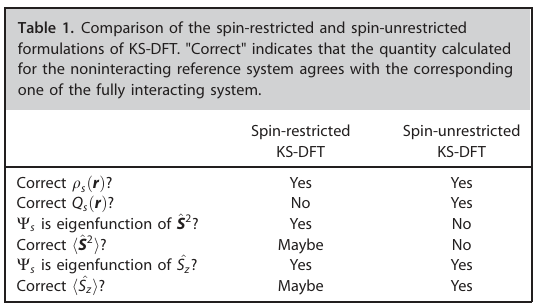
\includegraphics[width=0.9\linewidth]{tabla1.png}
    \caption{Comparison of the spin-restricted and spin-unrestricted
 formulations of KS-DFT. "Correct" indicates that the quantity calculated
 for the noninteracting reference system agrees with the corresponding
 one of the fully interacting system}
    \label{fig:enter-label1}
\end{figure}

This figure \ref{fig:enter-label1} compares spin-restricted and spin-unrestricted KS-DFT formulations. It shows that both correctly reproduce the total density \( \rho_s(r) \), but only the unrestricted formulation matches the spin density \( Q_s(r) \) of the interacting system. The restricted wavefunction \( \Psi_s \) is always an eigenfunction of \( \hat{S}^2 \), though its eigenvalue may not be correct. In the unrestricted case, \( \Psi_s \) is not an eigenfunction of \( \hat{S}^2 \), but it correctly reproduces \( \langle \hat{S}_z^2 \rangle \).
 
\begin{figure}[H]
    \centering
    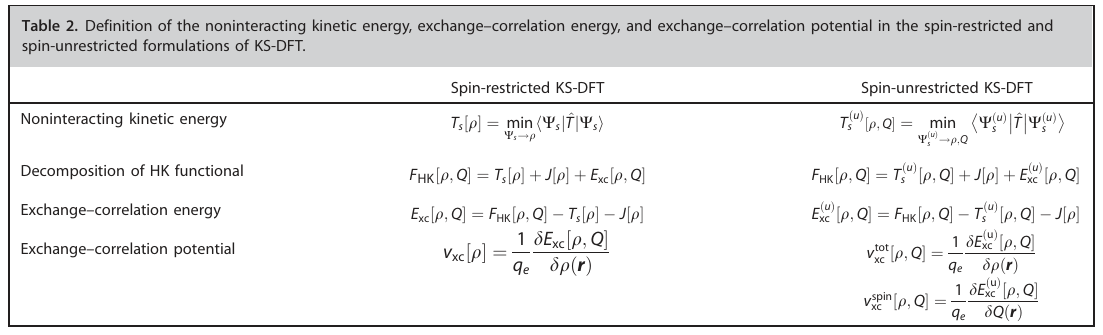
\includegraphics[width=1.1\linewidth]{tabla2.png}
    \caption{Definition of the noninteracting kinetic energy, exchange–correlation energy, and exchange–correlation potential in the spin-restricted and
 spin-unrestricted formulations of KS-DFT.}
    \label{fig:enter-label2}
\end{figure}

This figure \ref{fig:enter-label2} outlines the key definitions in spin-restricted and spin-unrestricted KS-DFT formulations. The noninteracting kinetic energy \( T_s[\rho] \) in the restricted case depends only on the total density, while \( T_s^{(u)}[\rho, Q] \) in the unrestricted case accounts for spin density as well. The Hohenberg-Kohn (HK) functional decomposition includes \( T_s \), the classical Coulomb term \( J[\rho] \), and the exchange-correlation energy \( E_{xc} \), which differs in formulation for both cases. The exchange-correlation potential \( v_{xc}[\rho] \) in the restricted formulation acts on total density, whereas the unrestricted formulation introduces an additional spin potential \( v_{xc}^{\text{spin}}[\rho, Q] \), acting on the spin density.
Defines the non-interacting kinetic energy, exchange-correlation energy, and exchange-correlation potential for the two formulations. These tables offer a concise overview of the essential distinctions and provide a clear comparison of the practical implications of each approach.
%\tableofcontents


\section{Conclusion}
Incorporating spin into density functional theory is essential to accurately describe electronic systems, especially in contexts where magnetic interactions and spin states play a dominant role. This work has highlighted theoretical advances, such as the generalization of the Hohenberg–Kohn theorems to spin-dependent systems, and computational challenges, including spin contamination in unrestricted formulations.

It is concluded that, although current DFT approximations have proven useful, they present significant limitations in the description of open-shell systems and fractional spin states. The lack of energy invariance in these cases introduces errors that must be corrected by developing more robust and specific functionals for spin-dependent systems.

Finally, this analysis underlines the importance of addressing these challenges through a combination of theoretical advances and computational improvements, which will allow a more accurate treatment of spin and, consequently, a deeper understanding of the electronic and magnetic properties of materials.

\begin{equation}
    \rho(\mathbf{r}) = \rho_{\alpha}(\mathbf{r}) + \rho_{\beta}(\mathbf{r})
\end{equation}

\subsubsection{Citations}

\begin{thebibliography}{144}
\bibitem{Jeschke2007} G. Jeschke, Y. Polyhach, \textit{Phys. Chem. Chem. Phys.} \textbf{2007}, \textit{9}, 1895.
\bibitem{Herrmann2010} C. Herrmann, G. C. Solomon, M. A. Ratner, \textit{J. Am. Chem. Soc.} \textbf{2010}, \textit{132}, 3682.
\bibitem{Herrmann2011} C. Herrmann, G. C. Solomon, M. A. Ratner, \textit{J. Chem. Phys.} \textbf{2011}, \textit{134}, 224306.
\bibitem{Timco2009} G. A. Timco, S. Carretta, F. Troiani, F. Tuna, R. J. Pritchard, C. A. Muryn, E. J. L. McInnes, A. Ghirri, A. Candini, P. Santini, G. Amoretti, M. Affronte, R. E. P. Winpenny, \textit{Nat. Nanotech.} \textbf{2009}, \textit{4}, 173.
\bibitem{McEvoy2006} J. P. McEvoy, G. W. Brudvig, \textit{Chem. Rev.} \textbf{2006}, \textit{106}, 4455.
\bibitem{Vignais2007} P. M. Vignais, B. Billoud, \textit{Chem. Rev.} \textbf{2007}, \textit{107}, 4206.
\bibitem{Stiebritz2012} M. T. Stiebritz, M. Reiher, \textit{Chem. Sci.} \textbf{2012}, \textit{3}, 1739.
\bibitem{Hu2010} Y. Hu, M. W. Ribbe, \textit{Acc. Chem. Res.} \textbf{2010}, \textit{43}, 475.
\bibitem{Schroder2000} D. Schr\"oder, S. Shaik, H. Schwarz, \textit{Acc. Chem. Res.} \textbf{2000}, \textit{33}, 139.
\bibitem{Helgaker2000} T. Helgaker, P. J\o rgensen, J. Olsen, \textit{Molecular Electronic Structure Theory}; Wiley: Chichester, 2000.
\bibitem{Koch2001} W. Koch, M. C. Holthausen, \textit{A Chemist’s Guide to Density Functional Theory}, 2nd ed.; Wiley-VCH: Weinheim, 2001.
\bibitem{Reiher2009} M. Reiher, \textit{Chimia} \textbf{2009}, \textit{63}, 140.
\bibitem{Roos2008} B. O. Roos, V. Veryazov, J. Conradie, P. R. Taylor, A. Ghosh, \textit{J. Phys. Chem. B} \textbf{2008}, \textit{112}, 14099.
\bibitem{Radon2008} M. Radon, K. Pierloot, \textit{J. Phys. Chem. A} \textbf{2008}, \textit{112}, 11824.
\bibitem{Radon2010} M. Radon, E. Broclawik, K. Pierloot, \textit{J. Phys. Chem. B} \textbf{2010}, \textit{114}, 1518.
\bibitem{Sala2010} X. Sala, M. Z. Ertem, L. Vigara, T. K. Todorova, W. Chen, R. C. Rocha, F. Aquilante, C. J. Cramer, L. Gagliardi, A. Llobet, \textit{Angew. Chem. Int. Ed.} \textbf{2010}, \textit{49}, 7745.
\bibitem{Planas2011} N. Planas, L. Vigara, C. Cady, P. Miro, P. Huang, L. Hammarstr\"om, S. Styring, N. Leidel, H. Dau, M. Haumann, L. Gagliardi, C. J. Cramer, A. Llobet, \textit{Inorg. Chem.} \textbf{2011}, \textit{50}, 11134.
\bibitem{Vigara2012} L. Vigara, M. Z. Ertem, N. Planas, F. Bozoglian, N. Leidel, H. Dau, M. Haumann, L. Gagliardi, C. J. Cramer, A. Llobet, \textit{Chem. Sci.} \textbf{2012}, \textit{3}, 2576.
\bibitem{Chan2010} G. K.-L. Chan, J. J. Dorando, D. Ghosh, J. Hachmann, \textit{Phys. Chem. Chem. Phys.} \textbf{2010}, \textit{13}, 6750.
\bibitem{Marti2011} K. H. Marti, M. Reiher, \textit{Phys. Chem. Chem. Phys.} \textbf{2011}, \textit{13}, 6750.
\bibitem{Frenking2000} G. Frenking, N. Fr\"ohlich, \textit{Chem. Rev.} \textbf{2000}, \textit{100}, 717.
\bibitem{Ziegler2005} T. Ziegler, J. Autschbach, \textit{Chem. Rev.} \textbf{2005}, \textit{105}, 2695.
\bibitem{Neese2009} F. Neese, \textit{Coord. Chem. Rev.} \textbf{2009}, \textit{253}, 526.
\bibitem{Podewitz2010} M. Podewitz, M. Reiher, \textit{Adv. Inorg. Chem.} \textbf{2010}, \textit{62}, 177.
\bibitem{Podewitz2011} M. Podewitz, T. Weymuth, M. Reiher, In \textit{Modeling of Molecular Properties}; P. Comba, Ed.; Wiley-VCH: Weinheim, 2011; pp. 137–163.
\bibitem{Ghosh2006} A. Ghosh, \textit{J. Biol. Inorg. Chem.} \textbf{2006}, \textit{11}, 671.
\bibitem{Cramer2009} C. J. Cramer, D. G. Truhlar, \textit{Phys. Chem. Chem. Phys.} \textbf{2009}, \textit{11}, 10757.
\bibitem{Reiher2001} M. Reiher, O. Salomon, B. A. Hess, \textit{Theor. Chem. Acc.} \textbf{2001}, \textit{107}, 48.
\bibitem{Reiher2002} M. Reiher, \textit{Inorg. Chem.} \textbf{2002}, \textit{41}, 6928.
\bibitem{Ghosh2003} A. Ghosh, P. R. Taylor, \textit{Curr. Opin. Chem. Biol.} \textbf{2003}, \textit{7}, 113.
\bibitem{Harvey2004} J. N. Harvey, \textit{Struct. Bond.} \textbf{2004}, \textit{112}, 151.
\bibitem{Herrmann2006} C. Herrmann, L. Yu, M. Reiher, \textit{J. Comput. Chem.} \textbf{2006}, \textit{27}, 1223.
\bibitem{Swart2008} M. Swart, \textit{J. Chem. Theory Comput.} \textbf{2008}, \textit{4}, 2057.
\bibitem{Ye2010} S. Ye, F. Neese, \textit{Inorg. Chem.} \textbf{2010}, \textit{49}, 772.
\bibitem{Swart2012} M. Swart, \textit{Int. J. Quantum Chem.} (in press). DOI: 10.1002/qua.24255



\bibitem{Ye2010} S. Ye, F. Neese, \textit{Inorg. Chem.}, 2010, \textbf{49}, 772.

\bibitem{Swart} M. Swart, \textit{Int. J. Quantum Chem.}, (in press). DOI: 10.1002/qua.24255.

\bibitem{Conradie2007} J. Conradie, A. Ghosh, \textit{J. Phys. Chem. B}, 2007, \textbf{111}, 12621.

\bibitem{Boguslawski2011} K. Boguslawski, Ch. R. Jacob, M. Reiher, \textit{J. Chem. Theory Comput.}, 2011, \textbf{7}, 2740.

\bibitem{Boguslawski2012} K. Boguslawski, K. H. Marti, O. Legeza, M. Reiher, \textit{J. Chem. Theory Comput.}, 2012, \textbf{8}, 1970.

\bibitem{Noodleman1981} L. Noodleman, \textit{J. Chem. Phys.}, 1981, \textbf{74}, 5737.

\bibitem{Jonkers1982} G. Jonkers, C. A. de Lange, L. Noodleman, E. J. Baerends, \textit{Mol. Phys.}, 1982, \textbf{46}, 609.

\bibitem{Noodleman1985} L. Noodleman, J. G. Norman, J. H. Osborne, A. Aizman, D. A. Case, \textit{J. Am. Chem. Soc.}, 1985, \textbf{107}, 3418.

\bibitem{Noodleman1986} L. Noodleman, E. R. Davidson, \textit{Chem. Phys.}, 1986, \textbf{109}, 131.

\bibitem{Reiher2007} M. Reiher, \textit{Faraday Discuss.}, 2007, \textbf{135}, 97.

\bibitem{Noodleman1995} L. Noodleman, C. Y. Peng, D. A. Case, J. M. Mouesca, \textit{Coord. Chem. Rev.}, 1995, \textbf{144}, 199.

\bibitem{vanWullen2009} C. van Wüllen, \textit{J. Phys. Chem. A}, 2009, \textbf{113}, 11535.

\bibitem{Pantazis2009} D. A. Pantazis, M. Orio, T. Petrenko, S. Zein, E. Bill, W. Lubitz, J. Messinger, F. Neese, \textit{Chem. Eur. J.}, 2009, \textbf{15}, 5108.

\bibitem{Schinzel2010} S. Schinzel, J. Schraut, A. V. Arbuznikov, P. E. M. Siegbahn, M. Kaupp, \textit{Chem. Eur. J.}, 2010, \textbf{16}, 10424.

\bibitem{Cohen2012} A. J. Cohen, P. Mori-Sanchez, W. Yang, \textit{Chem. Rev.}, 2012, \textbf{112}, 289.

\bibitem{Parr1989} R. G. Parr, W. Yang, \textit{Density-Functional Theory of Atoms and Molecules}, Oxford University Press: Oxford, 1989.

\bibitem{Gross1990} E. K. U. Gross, R. M. Dreizler, \textit{Density Functional Theory: An Approach to the Quantum Many-Body Problem}, Springer: Berlin, 1990.

\bibitem{Fiolhais2003} C. Fiolhais, F. Nogueira, M. A. L. Marques, \textit{A Primer in Density Functional Theory}, Lecture Notes in Physics; Springer: Berlin, 2003.

\bibitem{Engel2011} E. Engel, R. M. Dreizler, \textit{Density Functional Theory: An Advanced Course}, Springer: Heidelberg, 2011.

\bibitem{Ye2010} S. Ye, F. Neese, \textit{Inorg. Chem.}, 2010, \textbf{49}, 772.

\bibitem{Swart} M. Swart, \textit{Int. J. Quantum Chem.}, (in press). DOI: 10.1002/qua.24255.

\bibitem{Conradie2007} J. Conradie, A. Ghosh, \textit{J. Phys. Chem. B}, 2007, \textbf{111}, 12621.

\bibitem{Boguslawski2011} K. Boguslawski, Ch. R. Jacob, M. Reiher, \textit{J. Chem. Theory Comput.}, 2011, \textbf{7}, 2740.

\bibitem{Boguslawski2012} K. Boguslawski, K. H. Marti, O. Legeza, M. Reiher, \textit{J. Chem. Theory Comput.}, 2012, \textbf{8}, 1970.

\bibitem{Noodleman1981} L. Noodleman, \textit{J. Chem. Phys.}, 1981, \textbf{74}, 5737.

\bibitem{Jonkers1982} G. Jonkers, C. A. de Lange, L. Noodleman, E. J. Baerends, \textit{Mol. Phys.}, 1982, \textbf{46}, 609.

\bibitem{Noodleman1985} L. Noodleman, J. G. Norman, J. H. Osborne, A. Aizman, D. A. Case, \textit{J. Am. Chem. Soc.}, 1985, \textbf{107}, 3418.

\bibitem{Noodleman1986} L. Noodleman, E. R. Davidson, \textit{Chem. Phys.}, 1986, \textbf{109}, 131.

\bibitem{Reiher2007} M. Reiher, \textit{Faraday Discuss.}, 2007, \textbf{135}, 97.

\bibitem{Noodleman1995} L. Noodleman, C. Y. Peng, D. A. Case, J. M. Mouesca, \textit{Coord. Chem. Rev.}, 1995, \textbf{144}, 199.

\bibitem{vanWullen2009} C. van Wüllen, \textit{J. Phys. Chem. A}, 2009, \textbf{113}, 11535.

\bibitem{Pantazis2009} D. A. Pantazis, M. Orio, T. Petrenko, S. Zein, E. Bill, W. Lubitz, J. Messinger, F. Neese, \textit{Chem. Eur. J.}, 2009, \textbf{15}, 5108.

\bibitem{Schinzel2010} S. Schinzel, J. Schraut, A. V. Arbuznikov, P. E. M. Siegbahn, M. Kaupp, \textit{Chem. Eur. J.}, 2010, \textbf{16}, 10424.

\bibitem{Cohen2012} A. J. Cohen, P. Mori-Sanchez, W. Yang, \textit{Chem. Rev.}, 2012, \textbf{112}, 289.

\bibitem{Parr1989} R. G. Parr, W. Yang, \textit{Density-Functional Theory of Atoms and Molecules}, Oxford University Press: Oxford, 1989.

\bibitem{Gross1990} E. K. U. Gross, R. M. Dreizler, \textit{Density Functional Theory: An Approach to the Quantum Many-Body Problem}, Springer: Berlin, 1990.

\bibitem{Fiolhais2003} C. Fiolhais, F. Nogueira, M. A. L. Marques, \textit{A Primer in Density Functional Theory}, Lecture Notes in Physics; Springer: Berlin, 2003.

\bibitem{Engel2011} E. Engel, R. M. Dreizler, \textit{Density Functional Theory: An Advanced Course}, Springer: Heidelberg, 2011.

\bibitem{Zheludev1994} A. Zheludev, V. Barone, M. Bonnet, B. Delley, A. Grand, E. Ressouche, P. Rey, R. Subra, J. Schweizer, \textit{J. Am. Chem. Soc.}, 1994, \textbf{116}, 2019.

\bibitem{Baron1996} V. Baron, B. Gillon, O. Plantevin, A. Cousson, C. Mathoniere, O. Kahn, A. Grand, L. Öhrström, B. Delley, \textit{J. Am. Chem. Soc.}, 1996, \textbf{118}, 11822.

\bibitem{Pontillon1999} Y. Pontillon, A. Caneschi, D. Gatteschi, R. Sessoli, E. Ressouche, J. Schweizer, E. Lelievre-Berna, \textit{J. Am. Chem. Soc.}, 1999, \textbf{121}, 5342.

\bibitem{Claiser2005} N. Claiser, M. Souhassou, C. Lecomte, B. Gillon, C. Carbonera, A. Caneschi, A. Dei, D. Gatteschi, A. Bencini, Y. Pontillon, E. Lelievre-Berna, \textit{J. Phys. Chem. B}, 2005, \textbf{109}, 2723.

\bibitem{Zaharko2010} O. Zaharko, P. J. Brown, M. Mys’kiv, \textit{Phys. Rev. B}, 2010, \textbf{81}, 172405.

\bibitem{McWeeny1961} R. McWeeny, Y. Mizuno, \textit{Proc. Roy. Soc. Ser. A}, 1961, \textbf{259}, 554.

\bibitem{Davidson1976} E. R. Davidson, \textit{Reduced Density Matrices in Quantum Chemistry}, Academic Press: New York, 1976.

\bibitem{Mazziotti2011} D. A. Mazziotti, \textit{Chem. Rev.}, 2011, \textbf{112}, 244.

\bibitem{Hohenberg1964} P. Hohenberg, W. Kohn, \textit{Phys. Rev.}, 1964, \textbf{136}, B864.

\bibitem{Levy1979} M. Levy, \textit{Proc. Natl. Acad. Sci. USA}, 1979, \textbf{76}, 6062.

\bibitem{Perdew1982} J. P. Perdew, R. G. Parr, M. Levy, J. L. Balduz, Jr., \textit{Phys. Rev. Lett.}, 1982, \textbf{49}, 1691.

\bibitem{Lieb1983} E. H. Lieb, \textit{Int. J. Quantum Chem.}, 1983, \textbf{24}, 243.

\bibitem{Leeuwen2003} R. van Leeuwen, \textit{Adv. Quantum Chem.}, 2003, \textbf{43}, 25.

\bibitem{Eschrig2003} H. Eschrig, \textit{The Fundamentals of Density Functional Theory}, 2nd ed.; Eagle, Ed. am Gutenbergplatz: Leipzig, 2003.

\bibitem{Kohn1985} W. Kohn, In \textit{Highlights of Condensed-Matter Theory}, F. Bassani, F. Fumi, M. P. Tosi, Eds.; Elsevier: Amsterdam, 1985, pp. 1–15.

\bibitem{Perdew2009} J. P. Perdew, A. Ruzsinszky, L. A. Constantin, J. Sun, G. I. Csonka, \textit{J. Chem. Theory Comput.}, 2009, \textbf{5}, 902.

\bibitem{Perdew1981} J. P. Perdew, A. Zunger, \textit{Phys. Rev. B}, 1981, \textbf{23}, 5048.

\bibitem{Barth1972} U. von Barth, L. Hedin, \textit{J. Phys. C: Solid State Phys.}, 1972, \textbf{5}, 1629.

\bibitem{Ayers2006} P. W. Ayers, W. Yang, \textit{J. Chem. Phys.}, 2006, \textbf{124}, 224108.

\bibitem{Holas2006} A. Holas, R. Balawender, \textit{J. Chem. Phys.}, 2006, \textbf{125}, 247101.

\bibitem{Eschrig2001} H. Eschrig, W. E. Pickett, \textit{Solid State Commun.}, 2001, \textbf{118}, 123.

\bibitem{Capelle2001} K. Capelle, G. Vignale, \textit{Phys. Rev. Lett.}, 2001, \textbf{86}, 5546.

\bibitem{Gal2010a} T. Gal, P. Geerlings, \textit{Phys. Rev. A}, 2010, \textbf{81}, 032512.

\bibitem{Gal2010b} T. Gal, P. Geerlings, \textit{J. Chem. Phys.}, 2010, \textbf{133}, 144105.

\bibitem{Gidopoulos2007} N. I. Gidopoulos, \textit{Phys. Rev. B}, 2007, \textbf{75}, 134408.

\bibitem{Gal2007} T. Gal, \textit{Phys. Rev. B}, 2007, \textbf{75}, 235119.

\bibitem{Gal2009} T. Gal, P. W. Ayers, F. De Proft, P. Geerlings, \textit{J. Chem. Phys.}, 2009, \textbf{131}, 154114.

\bibitem{Yang2000} W. Yang, Y. Zhang, P. W. Ayers, \textit{Phys. Rev. Lett.}, 2000, \textbf{84}, 5172.

\bibitem{Cohen2008a} A. J. Cohen, P. Mori-Sanchez, W. Yang, \textit{Science}, 2008, \textbf{321}, 792.

\bibitem{Cohen2008b} A. J. Cohen, P. Mori-Sanchez, W. Yang, \textit{J. Chem. Phys.}, 2008, \textbf{129}, 121104.

\bibitem{Gunnarsson1976} O. Gunnarsson, B. I. Lundqvist, \textit{Phys. Rev. B}, 1976, \textbf{13}, 4274.

\bibitem{Wang2000} Y. A. Wang, E. A. Carter, In \textit{Theoretical Methods in Condensed Phase Chemistry}, S. D. Schwartz, Ed.; Kluwer: Dordrecht, 2000, pp. 117–184.

\bibitem{Xia2012} J. Xia, C. Huang, I. Shin, E. A. Carter, \textit{J. Chem. Phys.}, 2012, \textbf{136}, 084102.

\bibitem{Kohn1965} W. Kohn, L. J. Sham, \textit{Phys. Rev.}, 1965, \textbf{140}, A1133.

\bibitem{Levy1982} M. Levy, \textit{Phys. Rev. A}, 1982, \textbf{26}, 1200.
\bibitem{Schipper1998} P. R. T. Schipper, O. V. Gritsenko, E. J. Baerends, \textit{Theor. Chem. Acc.}, 1998, \textbf{99}, 329.

\bibitem{Morrison2002} R. C. Morrison, \textit{J. Chem. Phys.}, 2002, \textbf{117}, 10506.

\bibitem{Katriel2004} J. Katriel, S. Roy, M. Springborg, \textit{J. Chem. Phys.}, 2004, \textbf{121}, 12179.

\bibitem{Pople1995} J. A. Pople, P. M. W. Gill, N. C. Handy, \textit{Int. J. Quantum Chem.}, 1995, \textbf{56}, 303.

\bibitem{Chipman1983} D. M. Chipman, \textit{J. Chem. Phys.}, 1983, \textbf{78}, 3112.

\bibitem{Chipman1992} D. M. Chipman, \textit{Theor. Chem. Acc.}, 1992, \textbf{82}, 93.

\bibitem{Wang1995} J. Wang, A. D. Becke, V. H. Smith, Jr., \textit{J. Chem. Phys.}, 1995, \textbf{102}, 3477.

\bibitem{Cohen2007} A. J. Cohen, D. J. Tozer, N. C. Handy, \textit{J. Chem. Phys.}, 2007, \textbf{126}, 214104.

\bibitem{Daul1994} C. Daul, \textit{Int. J. Quantum Chem.}, 1994, \textbf{52}, 867.

\bibitem{Daul1995} C. A. Daul, K. G. Doclo, A. C. Stückl, In \textit{Recent Advances in Density Functional Methods, Part 2}; D. P. Chong, Ed.; World Scientific: Singapore, 1995, pp. 61–113.

\bibitem{Filatov1998} M. Filatov, S. Shaik, \textit{Chem. Phys. Lett.}, 1998, \textbf{288}, 689.

\bibitem{Filatov1999} M. Filatov, S. Shaik, \textit{Chem. Phys. Lett.}, 1999, \textbf{304}, 429.

\bibitem{Illas2006} F. Illas, I. Moreira, J. Bofill, M. Filatov, \textit{Theor. Chem. Acc.}, 2006, \textbf{116}, 587.

\bibitem{Frank1998} I. Frank, J. Hutter, D. Marx, M. Parrinello, \textit{J. Chem. Phys.}, 1998, \textbf{108}, 4060.

\bibitem{Grimm2003a} S. Grimm, C. Nonnenberg, I. Frank, \textit{J. Chem. Phys.}, 2003, \textbf{119}, 11574.

\bibitem{Nonnenberg2003} C. Nonnenberg, S. Grimm, I. Frank, \textit{J. Chem. Phys.}, 2003, \textbf{119}, 11585.

\bibitem{DellaSala2003} F. Della Sala, A. Görling, \textit{J. Chem. Phys.}, 2003, \textbf{118}, 10439.

\bibitem{Vitale2005} V. Vitale, F. Della Sala, A. Görling, \textit{J. Chem. Phys.}, 2005, \textbf{122}, 244102.

\bibitem{Bagus1975} P. S. Bagus, B. I. Bennett, \textit{Int. J. Quantum Chem.}, 1975, \textbf{9}, 143.

\bibitem{Ziegler1977} T. Ziegler, A. Rauk, E. J. Baerends, \textit{Theor. Chim. Acta}, 1977, \textbf{43}, 261.

\bibitem{Perdew1995} J. P. Perdew, A. Savin, K. Burke, \textit{Phys. Rev. A}, 1995, \textbf{51}, 4531.

\bibitem{Fux2012} S. Fux, M. Reiher, \textit{Struct. Bond.}, 2012, \textbf{147}, 99.

\bibitem{Rajagopal1973} A. K. Rajagopal, J. Callaway, \textit{Phys. Rev. B}, 1973, \textbf{7}, 1912.

\bibitem{MacDonald1979} A. H. MacDonald, S. H. Vosko, \textit{J. Phys. C: Solid State Phys.}, 1979, \textbf{12}, 2977.

\bibitem{Engel2002} E. Engel, In \textit{Relativistic Electronic Structure Theory Part 1: Fundamentals}, P. Schwerdtfeger, Ed.; Elsevier: Amsterdam, 2002, pp. 523–621.

\bibitem{Engel2003} E. Engel, R. M. Dreizler, S. Varga, B. Fricke, In \textit{Relativistic Effects in Heavy-Element Chemistry and Physics}, B. A. Hess, Ed.; Wiley: Chichester, 2003, pp. 123–161.

\bibitem{Saue2002} T. Saue, T. Helgaker, \textit{J. Comput. Chem.}, 2002, \textbf{23}, 814.

\bibitem{Engel1996} E. Engel, R. Dreizler, \textit{Top. Curr. Chem.}, 1996, \textbf{181}, 1.

\bibitem{VanWullen2010} C. Van Wüllen, In \textit{Relativistic Methods for Chemists, Challenges and Advances in Computational Chemistry and Physics}; M. Barysz, Y. Ishikawa, Eds.; Springer: Dordrecht, 2010; pp. 191–214.

\bibitem{Baym1969} G. Baym, \textit{Lectures on Quantum Mechanics}; Benjamin–Cummings: New York, 1969.

\bibitem{VanWullen1999} C. Van Wüllen, \textit{J. Comput. Chem.}, 1999, \textbf{20}, 51.

\bibitem{VanWullen2002} C. Van Wüllen, \textit{J. Comput. Chem.}, 2002, \textbf{23}, 779.

\bibitem{Scalmani2012} G. Scalmani, M. J. Frisch, \textit{J. Chem. Theory Comput.}, 2012, \textbf{8}, 2193.

\bibitem{Peng2012} D. Peng, M. Reiher, \textit{Theor. Chem. Acc.}, 2012, \textbf{131}, 1081.

\bibitem{Mastalerz2008} R. Mastalerz, R. Lindh, M. Reiher, \textit{Chem. Phys. Lett.}, 2008, \textbf{465}, 157.

\bibitem{Baerends1997} E. J. Baerends, O. V. Gritsenko, \textit{J. Phys. Chem. A}, 1997, \textbf{101}, 5383.



\end{thebibliography}



\end{document}
%
% ****** End of file apssamp.tex ******
